\documentclass{article}
\usepackage[utf8]{inputenc}
\usepackage[nottoc]{tocbibind}
\usepackage{csquotes}
\usepackage{hyperref}
\usepackage{amsmath}
\usepackage{amssymb}
\usepackage{float}
\usepackage{amsthm}
\usepackage{appendix}
\usepackage[landau, sets, operators, probability, complexity, asymptotics]{cryptocode}



\title{Zero Knowledge Proofs \\ Theory and Applications}
\author{Giacomo Fenzi \\ University of St. Andrews\thanks{Thanks in particular to Prof. Stephen Linton and Dr. Louis Theran}}
\date{September 2019}

% Definition of \maketitle
\makeatletter         
\def\@maketitle{
\begin{center}
{\Huge \@title }\\[4ex] 
{\Large  \@author}\\[4ex] 
\@date\\[8ex]
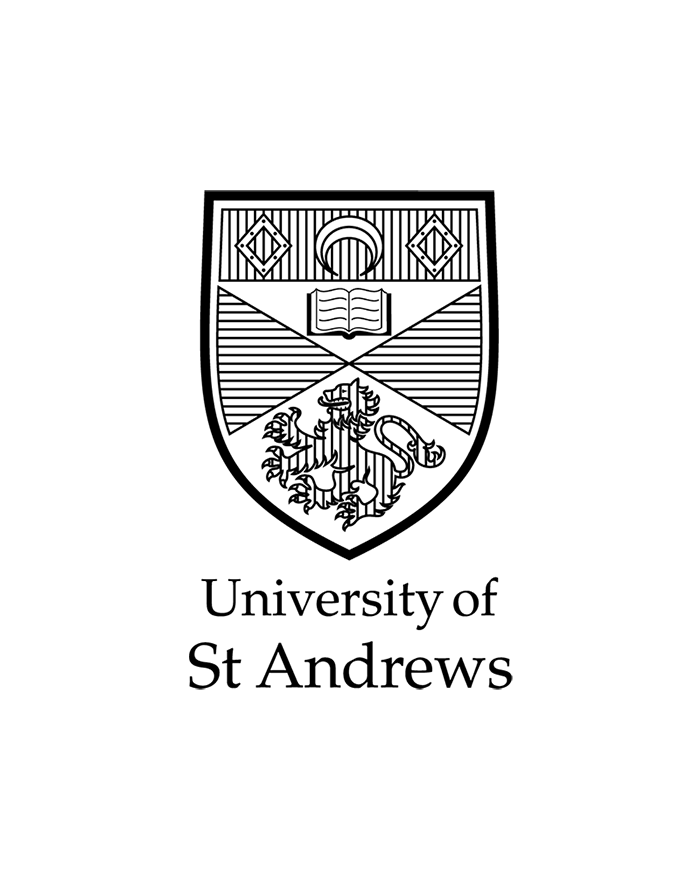
\includegraphics[width = 80mm]{uni_logo.png}
\end{center}}
\makeatother

\newtheorem{theorem}{Theorem}
\newtheorem{definition}{Definition}
\newtheorem{example}{Example}

\begin{document}

\maketitle
\newpage

\begin{abstract}
    In this paper we will provide a survey of the theory underlying Zero Knowledge Proofs,
    building up intuition for interactive proving protocol, which will then be formalized first in Interactive Proofs
    and then in more complex knowledge witholding schemes, such as Perfect and Computational Zero Knowledge Proofs.
    In the process, we will have shown interactive proofs for Graph Non Isomorphism (a co-$\npol$ problem),
    and zero knowledge proofs for both Graph Isomorphism and Graph 3-Colorability.
    Finally, we will detail some applications of the theory, showing various \enquote{flavours} of ZKP for the Discrete Logarithm problem that will culminate in
    Schnorr Signatures. We will compound this with the Secure Remote Protocol, a protocol that uses a similar ZKP in order
    to authenticate without communicating your password to the server. Finally, we show a very simple Zero Knowledge
    Range Proof, an instance of a very general class that has a wide range of applications and is currently one of the most active avenues of research.
    The paper will also introduce Sagemath worksheets that demonstrate nearly all of the protocols here detailed.
\end{abstract}

\section*{Declaration}
I declare that the material submitted for assessment is my own work except where credit is explicitly given to others
by citation or acknowledgement.
This work was performed during the current academic year except where otherwise stated.
The main text of this project report is 14896 words long, including project specification and plan.
In submitting this project report to the University of St Andrews, I give permission for it to be made available for use
in accordance with the regulations of the University Library. I also give permission for the report to be made
available on the Web, for this work to be used in research within the University of St Andrews,
and for any software to be released on an open source basis. I retain the copyright in this work, and ownership of any
resulting intellectual property.

\tableofcontents

\section{Introduction}
The concept of proof is one that resonates quite strongly in all of society. Having positive verification that
an untrusted party is actually making an affirmative claim opens up to a variety of avenues for collaboration and
enquiry. This paper will be a survey of the theory of a particular variety of proofs, namely Zero Knowledge Proofs.
We will build an understanding of Interactive Proofs, which are processes in which a verifier is successively convinced
by a prover. The fundamental idea is that the kind of proofs that we will consider are not fixed proofs as in Mathematics\footnote{They resemble mathematical proofs more closely when we consider Non Interactive Zero Knowledge Proofs},
but instead they are interactive processes, in which a verifier asks questions (or challenges) to the prover, and is progressively
convinced by correct answers.
The general problem that we look at is the following. Suppose that we have some object $x$ such that the proposition
$P(x)$ holds. How do we convince a skeptic of this fact? One way would be to just reveal $x$, but of course this
might not be desirable for a variety of reasons. For example, it might be that $x$ is a password, or contains other sensitive
information.  However, if $P(\cdot)$ has enough structure, we are able to devise a protocol in which the verifier can ask questions,
that the prover can only consistently answer if it indeed has $x$, and from which the verifier learns nothing about $x$,
except the fact that it exists. We will formalize such process, investigate the structure of the resulting class, and show some examples of protocols that satisfy said properties.
Finally, we will survey some applications of Zero Knowledge Proofs, in the fields of digital signatures and authentication.

\section{Structure}
The structure of the paper will be as following. Section \ref{motivation} will provide some motivation that show why
the effort of developing Zero Knowledge Proofs is justified. Section \ref{preliminaries} will cover the preliminaries,
that includes both the mathematical machinery needed and the definition of the computational settings that we will
be extensively using, namely that of Turing Machines. This Section will also introduce complexity classes that are
relevant to our analysis, such a $\pol, \npol, \bpp$, and introduce the concept of a proof in a computational sense.
Section \ref{proofreq} will explore this concept in more depths, exploring via examples the characterization of
Zero Knowledge Proofs, such as the general setup, soundness, completeness and the zero knowledge property.
Section \ref{interactiveproofs} will formalize the notion of proofs by introducting Interactive Turing Machine, and
introduce the wide class of interactive proofs, of which Zero Knowledge Proofs are a subset. We will then give an
example of an interactive proof for the Graph Non Isomorphism problem, complete with a proof of the fact.
In the following Section \ref{zkp} we will finally introduce Zero Knowledge Proofs, in both the perfect and computational
formulation. We will continue by providing an example of a Perfect Zero Knowledge Proof for deciding the Graph Isomorphism
language, and conclude the section by introducing bit commitments, and showing that if one way permutations\footnote{In fact this holds for one way functions as well, but the permutation proof is simpler} exist
then every language in $\npol$ has a Zero Knowledge Proof. This is done in Subsection \ref{np} by providing a
computational Zero Knowledge Proof for the $\npol$-complete problem of Graph 3-coloring.
In Section \ref{applications} we will then look at some applications, in three different context. First we will
show how we can use a ZKP for the Discrete Logarithm in order to digitally sign a message (Schnorr signatures). Secondly,
we will show how fundamentally similar proof can be used in order to implement an authentication scheme in which the
server never receives the user's password. Finally, we will show an extremely simple example of a Zero Knowledge Range
proof, which is a strategy by which a party can prove that a certain value that it knows is within a suitable range, while
maintaining anonimity to what that value actually is. This family of proofs have a far-reaching implication, as they allow
to implement complex systems upholding invariants while maintaining anonimity, such as payment systems or goverment sanctioned
age verification. Finally, Section \ref{implementation} will refer the reader to the Sage implementation of the proofs described
in the paper.

\section{Motivation}
\label{motivation}
Zero Knowledge Proofs have applications in a number of fields outside of theory.
Examples space from classical cryptography settings such as message signature and authentication to more
practical ones such as online age verification and electronic voting. The development\footnote{And the \enquote{hype} associated with it}
of online blockchain based transaction systems has given indications of another direction that ZKP applications could
emerge. In this section we will be focusing on this application, has it gives a good indication of a complex problem that
ZKP can solve. Consider a blockchain system, such as BitCoin\footnote{But not limited to, in fact, as far as I know, every major blockchain system works majorly in the same way}.
As you probably are aware, BitCoin accounts are uniquely identified
by an address, and this address is visible in every transaction that the account is involved in. In fact, knowing the ownership
of an account allows anyone to reconstruct from the public ledger the entire transaction history, complete with transaction
amounts. Furthermore, the balance of any address is publicly available. What some efforts are working on is to allow
for a blockchain system to be completely private, so that transactions can be done between actors while maintaining
anonimity. Of course, many technical problems arise when trying to do so, but let us focus on one in particular.
Suppose account $A$ wants to transfer an amount $X$ to an account $B$. What party $B$ would like to verify is that
$A$ actually has enough balance to transfer such amount. However, since the system that we design is private, $B$ does
not have the ability to peer into $A$ account or its balance. Instead, to solve this problem, we make it so that
when $A$ initiates the transaction, it produces a \enquote{proof} that its balance is greater than $X$.
This proof has to have three properties. First of all, it must be convincing, so that if $A$ does indeed have
enough funds, then $B$ will be confident that the proof provided is correct. Secondly, it must be
sound, so that if $A$ does not have enough funds $B$ will never be convinced that it does. Thirdly, it must
be zero knowledge, ensuring it will not leak to $B$ any information about $A$ (like balance, account number ecc.) other
than the fact that $A$ has more than $X$ in its balance. This can be done via what is called a Zero Knowledge Range Proof,
of which we will see a very simple example in Section \ref{applications}.


\section{Preliminaries}
\label{preliminaries}
\subsection{Mathematical Notation}
We start by defining some crucial sets of strings\footnote{In general, the use of the $\cdot ^ *$ operator, also known as the \textit{Kleene Star} on a finite set of elements (also known as \textit{alphabet}) generates the set of all finite sequences of elements of the original set. We don not make too much use of it in this text though}.
\begin{definition}
    $\bin^n = \set{ a_1 a_2 \dots a_n \mid a_i \in \bin}$
\end{definition}
\begin{definition}
    $\bin^* = \set{ a_1 a_2 \dots a_n \mid a_i \in \bin \text{ \normalfont{ and }} n \in \NN }$
\end{definition}

It is important to stress that $\bin^*$ is the set of all \textit{finite} strings, and also that the empty string, denoted $\epsilon \in \bin^*$.

\begin{definition}
    A \textbf{language} $L$ is a subset of $\bin^*$, i.e. $L \subseteq \bin^*$
\end{definition}

Examples of languages include
\[ \set{ x \in \bin^* \mid |x| = 2 }, \set{ \langle(x, y, z)\rangle \mid x^2 + y^2 = z^2 }, \dots \]
Note in particular the use of $\langle \cdot \rangle$ to denote the binary representation of the inner element. In general, as long as the element can be encoded in binary in polynomial space, we will not concern ourselves too much with said representation, and sometime even omit the brackets. In particular note that, unless specified otherwise, integers are encoded in binary and without brackets.  \par

Now, a couple of utilities for talking about the asymptotic complexity of various functions.

\begin{definition} We define the following sets:
    \begin{align*}
        \bigO{f}      & = \set{ g \mid \exists r \in \RR^+, N \in \NN \text{ s.t } \forall n \geq N : g(n) \leq r f(n)  }                       \\
        \bigOmega{f}  & = \set{ g \mid \exists r \in \RR^+, N \in \NN \text{ s.t } \forall n \geq N : r g(n) \geq f(n)  }                       \\
        \bigsmallO{f} & = \set{ g \mid \exists r_1,r_2 \in \RR^+, N \in \NN \text{ s.t } \forall n \geq N : r_1 g(n) \leq f(n) \leq r_2 g(n)  }
    \end{align*}
\end{definition}
We also allow for two slight relaxation of notation, writing for example $\bigO{f}$ as $\bigO{f(n)}$ and $f \in \bigO{g}$ as $f = \bigO{g}$. Furthermore, we define the following useful set:
\begin{definition} We define
    \[\poly[] = \bigcup_{i = 0}^\infty \bigO{n^i}\]
    as the set of all functions bounded above by a polynomial.
\end{definition}
As before, we will allow a slight relaxation and use $\poly[\cdot]$ to specify some fixed but unspecified polynomial.

\begin{definition}
    Let $\mu : \NN \to \RR$. We say $\mu$ is \textbf{negligible} if for every positive $\poly[\cdot]$ there exists a $N \in \NN$ s.t for every $n > N$ we have:
    \[\mu(n) < \frac{1}{\poly}\]
\end{definition}
As an example, functions such as $2^{-n}$ or $n^{-n}$ are negligible. In particular the set of negligible functions is closed under multiplication by elements of $\poly$. This is significant, as we usually aim to have the attacker's success probability to be negligible, and this means that even repeating the attack polynomially many time will not create a non negligible threat. \par

There a couple of notions of probability that we will most likely need.
First of all, we will use the notation $x \sample A$ to say that $x$ is uniformly selected from the set $A$\footnote{Equivalently, when $A$ finite, we have defined a random variable $X$ such that for every $a \in A$ we have  $\prob{X = a} = \frac{1}{|A|} $}

\begin{definition}
    Suppose we have a series of $n$ independent event $X_i$, each one of them
    occurring with probability $\theta$. Then the probability of the total number of success $X$ being exactly equal to $k$ follows a binomial distribution and:
    \[ \prob{X = k} = \binom{n}{k} \theta^k (1 - \theta)^{n - k} \]
\end{definition}
In particular, we have that in those $n$ trials we expect $\expect{X} = n\theta$ events to occurr. This is useful, expecially since
we have that the probability of an event always occurring is $\prob{X = n} = \theta^n$. This will be useful especially
to  estimate the probability of some algorithm succeeding multiple times when it is not supposed to.
Note in particular that if a algorithm spuriosly succeeds with probability $\theta \in [0, 1)$ then $\prob{X = n}$ is a
negligible function of $n$. \par

The following definition will be used for having a compact notation for selecting permutations.

\begin{definition}
    We define the following set (group) of permutations over a certain set.
    \[ S_X = \{ f: X \to X | \text{ s.t. } f \text{ is a bijection} \} \]
\end{definition}

Finally, a lot of our examples will deal with graphs and isomorphisms on graphs.

\begin{definition}
    A \textbf{graph} $G = (V, E)$ is a pair of sets, where $V$ is referred to as the vertex set, and $E \subseteq V \times V$ is the set of edges.
\end{definition}

\begin{definition}
    Let $G_1 = (V_1, E_1)$ and $G_2 = (V_2, E_2)$. A bijection $\phi: V_1 \to V_2$ is an \textbf{isomorphism} between $G_1, G_2$ iff
    \[ (v, v') \in E_1 \implies (\phi(v), \phi(v')) \in E_2 \]
    In the case such an isomorphism exists, the two graphs are said to be isomorphic, and we write this as $G_1 \cong G_2$.
\end{definition}

Finally, we introduce the following useful notation, for the graph obtained by permuting all vertexes of another graph.
\begin{definition}
    Let $G = (V, E)$, and $\pi \in S_V$, i.e. a permutation on the set $V$. Then we define $\pi(G) = (V, E')$ where:
    \[ E' = \set{ (\pi(v), \pi(v')) | (v, v') \in E } \]
    Clearly, $G \cong \pi(G)$.
\end{definition}

\subsection{Computational Setting}
The computational model used in this paper is that of Turing Machines (TMs) \cite{turingComputableNumbersApplication1937}. We will not discuss the inner definition of deterministic and non deterministic TMs, as, within the category, changes in definition do not create more than polynomial slowdowns, and as such for all intents and purposes can be considered the same \cite{aroraComputationalComplexityModern2009}.

In particular, we will be providing an uniform probability based definition for the complexity classes. The traditional (and equivalent) definitions are in the appendix.

The Turing machine that we will be using have a slightly relaxed transition function, which allows for two different actions to be taken on the same step (as in a non deterministic machine). Also, for a polynomial time Turing Machine\footnote{The polynomial bound is required since in theory decisions taken early in the execution can effect the running time and such the length of the string. If the machine $M$ is always polynomial time we can then find a bound $p$ s.t. $\forall r, T(M_r(x))) \leq p(|x|) $, and as such having $r \in \bin^{p(|x|)}$ will be enough} $M$ we will write $M_r(x)$ for the output of $M$ on $x$, where $r$ is a binary string, where the $i$-th character specifies which action the machine should take on step $i$. We can then let $l$ be the maximum length that $r$ can take and define the probability of $M$ outputting $y$ on input $x$ to be:

\begin{definition} The probability of machine $M$ outputting $y$ on input $x$
    \[ \prob{M(x) = y} = \frac{|\set{r \in \bin^{l} \mid M_r(x) = y }|}{2^{l}}\]
\end{definition}

Using this definition, we can then define our complexity classes.

\begin{definition}
    We say that a language $L \in \pol$ if there exists a probabilistic polynomial time TM $M$ such that:
    \[x \in L \iff \prob{M(x) = 1} = 1\]
\end{definition}

The complexity class $\pol$ is the one we most closely associate with \enquote{efficient} computation. Notable examples of languages which belong in $\pol$ are finite languages, regular languages, context free languages, and more. For example, the following are all in $\pol$ :
\[ \set{(a_1, ... a_n) \, | \, n \in \NN \text{ and } a_i \leq a_{i+1} }\]
\[ \set{ p \,|\, p \in \NN \text{ and } p \text{ prime } }\]
\[ \set{ (a, b, c) \, | \, a^2 + b^2 = c^2 } \]

In general, a language being in $\pol$ implies there exists a machine such that all the computation paths recognize the input if the input is indeed in the language. \par

Compare this to the definition of $\npol$.

\begin{definition}
    We say that a language $L \in \npol$ if there exists a probabilistic polynomial time TM $M$ such that:
    \[x \in L \iff \prob{M(x) = 1} > 0\]
\end{definition}

The definition implies that there is at least one path for which the input is accepted. It is easy to see that $\pol \subseteq \npol$, but the question of $\pol =_? \npol$ is still open \cite{cookComplexityTheoremprovingProcedures1971} \cite{jaffeMillenniumGrandChallenge2006}. There are many $\npol$ problems that we believe do not belong in $\pol$, such as the following:

\[ \texttt{INT\_FACT} = \set{ (n, k) \, | \, \exists f : 1 < f < k \text { and } f \text{ divides } n}\]
\[ \texttt{SUB\_SUM} = \set{ G \subset_{fin} \ZZ \, | \, \exists S \subseteq G : \sum_{i \in S} i = 0  } \]
\[ \texttt{SAT} = \set{ \phi : \bin^n \to \bin \, | \, n \in \NN \text{ and } \exists a_1 \dots a_n : \phi(a_1, \dots a_n) = 1 } \]
\[ \texttt{GRAPH\_HOM} = \set{ (G, H) \, | \, \exists \phi : G \to H \text{ s.t. $\phi$ is a graph homomorphism} }\]

In particular, the last three languages are instances of $\npol$-complete problems, i.e. problems that are conceptually as hard as any problem in $\npol$ (more on this in the appendix). It is interesting to see that each of this problem involves some sort of search over an exponentially large possibility space, and the correctness can be easily verified by the result of such search. We associate thus $\npol$ class with problems that can be efficiently verified.

\begin{definition}
    We say that a language $L \in \bpp$ if there exists a probabilistic polynomial time TM $M$ such that the following hold
    \begin{enumerate}
        \item $x \in L \iff \prob{M(x) = 1} \geq \frac{2}{3}$
        \item $x \notin L \iff \prob{M(x) = 0} \geq \frac{2}{3}$
    \end{enumerate}
    In this case we say that $L$ is \textbf{recognizable in probabilistic polynomial time}
\end{definition}

Note in particular that we can replace\footnote{By running the machine multiples times and taking majority vote} the $\frac{2}{3}$ constant with $\frac{1}{2} + \epsilon$ for any $0 < \epsilon < \frac{1}{2}$.

$\bpp$ is referred to as the class of bounded polynomial time languages. It is evident that $\pol \subseteq \bpp$ but, while it is believed that the classes are equal, no proof was yet found. This class is significant, as it is intrinsically associated with efficient computation. This is because of a few factors, first of all because the probabilistic computation closely mimics the capabilities of general purpose computer, which can use the external environment as a source of randomness. Secondly, polynomial time computation is feasible, and, as long as Moore's law holds, modern computer can every year improve faster than one can increase the problem size\footnote{What I mean is, if an algorithm takes $\poly[|x|]$ steps, and on year $n$ a computer can perform $\bigO{2^n}$ steps, then by waiting a suitable and polynomial number of years the time needed
    decreases exponentially. E.g., suppose that a given problem takes $|x|^3$ steps to be solved, and on year 0 a computer can
    perform 1000 steps per year. Then in year 0 we can solve instances of size at most $|x| = 10$. However, suppose in year $n$ the
    power of the computer is given by $1000 \cdot 2^n$. This implies that in year $n$ we can handle instances of size $|x| = 10 \cdot 2^{n/3} $, which is exponential in $n$}.
Let us have an example to clarify how a probabilistic algorithm works:
\begin{example}

    \begin{figure}[H]
        \centering
        \fbox{%
            \procedure{Matrix Multiplication Probabilistic}{%
                \text{Inputs: } A \in \FF^{n \times m}, B \in \FF^{n \times k}, C \in \FF^{k \times m} \\
                x \sample \FF^m \\
                \pcreturn Ax =_? BCx
            }
        }
        \caption{Algorithm for checking Matrix Multiplication probabilistically}
        \label{matrixmultiplication}
    \end{figure}

    Consider three matrices, $A, B, C$ where $A \in \FF^{n \times m}$, $B \in \FF^{n \times k}$, $C \in \FF^{k \times m}$.
    We want to solve the question $A =_? B C$. Of course, in a deterministic setting, we can simply multiply the two matrices (taking $\bigO{nkm}$ steps) and compare it with the first (in $\bigO{nm}$ steps), in a total of $\bigO{nmk + nm}$ steps.
    We can do better if we allow for some probabilistic error. Take the following procedure (also in Figure \ref{matrixmultiplication}) :
    \begin{enumerate}
        \item Take a random vector $x \in \FF^m$
        \item Compute $Ax$ and $BCx$.
        \item Compare the two resulting vectors (in $\FF^n$). If they are the same return true, else return false.
    \end{enumerate}
    Computationally wise, this might require less calculations. Let's assume you can select a random $k$-vector in $\bigO{k}$ steps, then the first step is $\bigO{m}$, the two computations take respectively $\bigO{nm}$ and $\bigO{k (n + m)}$\footnote{This is optimized computing $B(Cx)$} and the comparison will be $\bigO{n}$. So in total the algorithm is $\bigO{nm + kn + mk + n}$. We claim that, trivially, if $A = BC$ then the algorithm always answer correctly. Furthermore if $A \neq BC$ then the algorithm answers correctly in the majority of cases. Let $D = BC$ Note that if the algorithm is to output incorrectly, it must be that $Ax = Dx$. Then it must be that $(A - D) x = 0$, and as such $x \in \ker(A - D)$. Note that $A - D \in \FF^{n \times m}$ and as such $A - D$ can be seen as a linear transformation from $\FF^m \to \FF^n$. The whole problem reduces to finding the probability that a vector picked at random belongs to the kernel of a linear transformation. Let $|\FF| = q$, the size of the underlying field\footnote{Note that in this case we assume the underlying field to be finite, the infinite case can also be handled but requires more thought}. First of all note that since $A \neq D$ at least one of the of the row of the matrix is non zero, and as such $\dim \ker (A - D) < m$. Since the size of any vector space $V$ over $\FF$ is $|V| = q^{\dim V}$, then the size of the kernel is at most $q^{m - 1}$. As such the probability of a random vector belonging to the kernel is at most $\frac{q^{m-1}}{q^m}=\frac{1}{q}$. We can then calculate that, repeating the algorithm $l$ times the probability of getting at least one vector not in the kernel is $1 - \left(\frac{1}{q}\right)^l$ and if we want to ensure that this probability is greater than $\frac{2}{3}$ we can then set:
    \[l > \frac{\log \frac{1}{3}}{\log \frac{1}{q}} = \frac{\log{3}}{\log{q}}\]

    Finally, we can see that repeating the procedure $l$ times\footnote{In fact, since $l < 1$ for $q > 3$, repetition is only really needed for the trivial field $\ZZ_2$} (call this algorithm $M$) will have the following result:
    \begin{itemize}
        \item $A = BC \implies \prob{M(A, B,C) = 1} = 1$
        \item $A \neq BC \implies \prob{M(A, B,C) = 0} > \frac{2}{3}$
    \end{itemize}

    Note that that brings the final complexity to $\bigO{l(nm + kn + mk + n)}$ so for some values of $l$ this might actually be slower than the deterministic algorithm.

\end{example}


\subsection{Adversarial Settings}
In cryptography, in order to achieve sound schemes, it is common to work in what is commonly referred to as an adversarial setting.
Intuitively, while aiming to prove the security of a cryptography protocol, it is not sufficient to prove the construction secure from a particular subset of attacks. Instead it is necessary for it to be secure in the wake of \textit{any} strategy that a sufficiently well endowed attacker might take. \par

The capability of the attacker will vary depending on the level of security that the protocol needs to be hold to. For example, the computational power that the adversary has will affect the class of problems that it can solve.
As an instance, if a construction relies on (hard) instances of an $\npol$-complete problem (and if $\pol \neq \npol$) then a deterministic polynomial time attacker will not be able to break the scheme, while one with non-deterministic polynomial resources will be able to\footnote{For the sake of the argument, say this problem is a decision problem, say $L$. Then, since $L \in \npol$ there exists a deterministically recognizable $R_L \subseteq \bin^* \times \bin^* $ s.t. $x \in L \iff \exists y \text{ s.t. } (x, y) \in R_L$ and $|y| = \poly[|x|]$. So a NDTM can, to solve $x \in_? L$ guess $y$ in a polynomial number of non deterministic steps, and check if $(x, y)$ belongs in $R_L$ }.

In general, the most strict level of security that we might require is that of information theoric security, which holds even in the case that
an attacker has infinite computational power. We will see that Perfect Zero Knowledge Proofs have an information theoretic flavour, even
though saying that they are secure against an infinitely powerful attacker might be a stretch\footnote{What I mean is that, in perfect ZKP the output of the interaction can be perfectly simulated by polynomial time prover, which is
    an information theoric level of accuracy. However, any ZKP usually deals with an underlying language that is only interesting when it is not
    decidable in polynomial time. For example, Graph Isomorphism is one of such problems. While we can devise a perfect ZKP for this problem, this
    does not mean that an unbounded computational attacker cannot decided the problem. It merely means that even a perfect attacker cannot
    understand whether it is in a simulation or a real interaction. On a less formal note though, we can see that the zero knowledge
    property still holds, as an unbounded attacker in a sense already has all of the knowledge, and as such it cannot gain any more!}.
After that level, we usually require that the attacker has computational capabilities that are bounded by a polynomial.
This quite closely mirrors the real world requirements for most schemes. We will see that Computational Zero Knowledge Proofs
have this kind of protection, as they rely on the concept of computational indistinguishability.


\subsection{Notion of Proof}
The notion of a proof has extremely overloaded meaning, as it used in many disparate fields. In particular, the notion of a proof in Mathematics most closely comes to mind and, while mathematical proofs and ZKP ultimately aim to ascertain the validity of a statement, the way that they achieve that result varies. In formal logic, a proof is a fixed sequence of steps (derivations) that, from commonly agreed statement (axioms), reach the statement that we are wanting to prove. In contrast, in a ZKP the process is a dynamic interaction between multiple parties, more akin to the notion of proof in law or debating.

\section{Proof Requirements}
\label{proofreq}
In order to start visualizing the concept of ZKP, we can start with a couple of toy examples that are helpful. Here and in the rest of text we will refer to the prover as Peggy and to the verifier as Victor.
\begin{example}
    Assume that Victor is completely colorblind\footnote{i.e. that he cannot distinguish object based on color alone}.
    Peggy wants to prove to Victor that she is not colorblind, so she devises an experiment.
    Peggy takes two balls completely identical, save for their colour, and gives them to Victor, one in his left and one in his right hand.
    Peggy asks Victor to put the balls behind his back, and to decide whether to swap them or not, without telling her.
    She then asks Victor to show the two balls.
    Peggy concludes by telling Victor whether he swapped the balls or not.\\
    This is a zero knowledge proof in the sense that:
    \begin{enumerate}
        \item If Peggy were colorblind, she would not be able to tell whether Victor switched the balls or not, and so the best she could do is guess, getting it right $\frac{1}{2}$ of the time\footnote{And as such repeating the experiment $n$ times will bring her probability of always guessing right to $\frac{1}{2^n}$}.
        \item If Peggy is not colorblind, she will be able to answer correctly every time, and thus convince Victor
        \item Victor does not learn anything else about his environment, apart from the fact that Peggy is not colorblind.
    \end{enumerate}
\end{example}

\begin{example}
    This example is due to Jean-Jacques Quisquater \cite{quisquaterHowExplainZeroknowledge1989}.
    Consider a cave shaped like a ring, with a single entrance.
    On the side opposite to the entrance, there is a gate that divides the cave into two.
    The gate can only be opened by a secret word, that only Peggy knows.
    Peggy wants to prove to Victor that she possesses this secret word, without of course letting him in on the secret.
    She devises an experiment as follows.
    She tells Victor to wait at the entrance of the cave, and she goes by one of the two possible paths (without letting Victor know which one she took) to the gate, where she can utter the secret word without being heard.
    Then she asks Victor to name one of the two paths, and she goes back trough the named path.
    As before:
    \begin{enumerate}
        \item If Peggy did not know the secret word, she would not be able to go back on a path different from the one she initially took, and as such has only a $\frac{1}{2}$ chance of getting it right.
        \item Instead, if Peggy does indeed know the secret word, she will be able to always take the path that Victor names, and as such convince him
        \item Furthermore, Victor does not gain any knowledge of the secret key, apart from the fact that Peggy knows it.
    \end{enumerate}
\end{example}

This illustrates the general idea of Zero Knowledge Proofs. The proof part is devised as an experiment or challenge from the verifier to the prover, that the prover can only answer by having the necessary piece of information or \enquote{power}. The prover cannot fool the verifier consistently and an honest prover and honest verifier will agree on the fact. Furthermore no new information is learned by the verifier. Also, if external observers were to have witnessed the exchange they would not be convinced of the fact (as Peggy and Victor could have coordinated their answers).
We seek to formalize this next.

\subsection{Parties in play}
In the sequel, we will have two parties interacting, the \textit{prover} and the \textit{verifier} that, as before, will be colloquially referred to as Peggy and Victor. In mathematical notation we will have $P, V$ always referring, respectively, to prover and verifier. As in math, we aim to have the verification procedure be as efficient as possible, while most of the computational burden will be placed on the prover. This in some way mirrors the alternative definition of $\npol$, as the class of all problems whose solution can be efficiently verified. Furthermore, it is crucial to understand that the verifier inherently does not trust the prover (otherwise there would not be need for the proof to be provided), and as such Victor will be skeptical of everything that Peggy says. The general situation will be Peggy and Victor having access to some common input, plus each one possibly having access to some additional private input, which will often be related from the shared input.

\subsection{Soundness}
The condition of soundness asserts that an honest verifier cannot be tricked into accepting a false statement by a possibly cheating prover. In the first example, this is equivalent to stating that, if Peggy is indeed colorblind, then she cannot convince Victor that she is not. In the second one, if Peggy were not to know the password to the gate, then she would not be able to convince Victor which will then not be fooled. It is important to note that in the above example we actually allow for a dishonest prover to be able to successfully fool Victor with a bounded above probability\footnote{And this probability can be made negligible thanks to repeating the experiment multiple times}.
\subsection{Completeness}
Conversely, the condition of completeness states that an honest prover will be able to convince an honest verifier of the veracity of the claim, if the claim is indeed true. So, moving back to the first example, Peggy will be able to prove she is not colorblind if that is indeed true and Victor acts honestly satisfying the protocol. While in the examples Victor is always positively convinced at the end of the interaction, this is not a strict requirement, instead (similarly as in Soundness) we just require the interaction to succeed with a strictly bounded below probability\footnote{And again this probability can be increased by repeating the experiment and taking the majority answer}. As an example of when this might be the case, consider the following \begin{example}
    Peggy claims that coffee tastes differently when brewed by an espresso machine compared to one made in a cup. Victor wants to verify that claim, so he brews a coffee choosing randomly between the two options (in way that Peggy does not see which is which). Peggy then tastes the coffee, and gives her opinion on how it was brewed. The experiment is repeated $n$ times\footnote{According to \cite{chambersChemIDplus0000302272XFSBVAOIAHNAPCNPVHKAFCSAN}, and assuming Peggy weighs around 70kg, we would not recommend for $n$ to be greater than 75-100}, and Victor is convinced if Peggy is right more than $c$ times, where $c$ depends on how certain we want to be of Peggy's ability.
\end{example}

This is the exact subject of hypothesis testing, in particular it reduces to the exact problem of finding whether a coin is biased. This can be modeled by a binomial distribution with mean $\mu = n/2$ and standard deviation $\sigma = \frac{\sqrt{n}}{2}$. In particular, if we apply the central limit theorem (and as such have $n > 30$) we can model it as a normal distribution, then using the $3\sigma$ rule\footnote{i.e. that three standard deviations include 99.7\% of the data} we can see that if $|c - \frac{n}{2}| \geq 3\frac{\sqrt{n}}{2}$ then we can affirm that with a more than 99\% chance Peggy can distinguish the two. For example, if we set $n = 100$ and Peggy guesses right more than $c = 65 = \frac{100}{2} + 3 \frac{\sqrt{100}}{2}$ times (or less than 35 times) then we can be certain that Peggy is truthful (and in the other case that she can distinguish it but for some reasons she is convinced the espresso machine coffee is brewed in cup and viceversa).

\subsection{Zero Knowledge}
Formalizing the notion of zero knowledge requires a bit more work. We would like to be able to say that in any interaction with the prover the verifier does not gain any knowledge that it did not posses already. That shifts the conversation to what it means to gain knowledge. Let us consider for example the interaction of a prover and a verifier with a common input of a suitably large graph. If the prover reveals to the verifier whether the graph is connected or Eulerian or the average degree of its vertexes then in a sense the verifier does not gain any knowledge, as these are all easily (polynomial time) computable without any additional information. Instead if the prover reveals whether the graph is Hamiltonian, or the chromatic number of the graph, or a $k$-coloring of it\footnote{And of course assuming $\pol \neq \npol$ and that the corresponding problems cannot be solved in polynomial time} then the verifier gains knowledge, as it would have not been able to answer that question itself using an efficient procedure. This gives us a hint of what gaining knowledge can entail. In particular, we say that the verifier gains knowledge from an interaction with the prover if, after the interaction, it can efficiently compute something which it would have not been able to do before. How to rigorously express this is non trivial, and we defer the discussion to the following sections.

\section{Proof Systems}
\label{interactiveproofs}
In our drive to formalize the intuition that we gained in the previous sections, we will start by extending the model of a Turing Machine to allow for two Turing Machines to interact. Then we will define formally interactive proofs and give examples.

\subsection{Interactive Turing Machine}
First of all, we can start by extending the traditional randomized Turing Machine. It is of note that in interactive Turing Machines (ITMs) we are almost never interested in the execution of a single machine, but rather in the interconnected operation of the two machines. As such, it makes it easier to describe the behaviour of a pair of ITMs rather than of a single one. First of all, with this model we aim to preserve the following notions:
\begin{itemize}
    \item Exclusivity, so that, before termination, exactly one of the two machines is executing at any point in time
    \item Privacy, so each of the two machines can withold some information from the other\footnote{In particular we require that each machine is able to keep the contents of its random tape private. There are some cases in which this requirement might be lifted, in so called public coin protocols, but we will not discuss them here}
    \item Communication, each of the two machines can choose to let some information (often related to their private information) to the other, using communication tapes
\end{itemize}
To fulfill those goals, we define a pair of interactive machines as follows:
\begin{definition}
    A pair of interactive Turing Machines $A, B$ have the following characteristics:
    \begin{itemize}
        \item Each machine is a randomized Turing machine in its own right i.e. it has an input tape, an output tape, and a random tape\footnote{This is an alternate equivalent definition of randomized Turing Machines, it just makes the explanation easier}.
        \item Neither machine can access the other's aforementioned tapes.
        \item The system has two additional tapes, called communications tapes. For the sake of the argument, call them $T_1, T_2$. $A$ can read from $T_1$ and write to $T_2$, while $B$ can write to $T_1$ and read from $T_2$.
        \item Each machine has an access to a number of additional switch states, $\delta_S$, where $S$ is a state of the machine in question. If a transition sets the state to one of these $\delta$-states, then the current machine becomes idle, and execution is resumed on the other machine. When execution is resumed on a machine, the state it is in depends on the last suspension. If it was suspended in state $\delta_S$, then it will resume execution in state $S$. Of course, if no suspension occurred, the machine will start from the initial state.
        \item The interconnected randomized Turing machine pair terminates when either of the two machines terminates.
        \item An interactive proof system runs on some common input, which is initially written on both machines' input tape.
        \item By convention, $A$ is initially running, and $B$ is idle.
    \end{itemize}
\end{definition}

It is to be noted that there is an alternative and ultimately equivalent model that allows each machine to have an additional private input tape, which allows for both machines to be polynomial time. For simplicity here we work with the definition with less tapes, but it is good to be aware of it.

Using the above definition, we can go and define notation for the output of an execution of a pair of ITMs.

\begin{definition}
    Let $A, B$ be interconnected randomized Turing machines, such that both $A$ and $B$ always terminate in finitely many steps. Then we define $\left<A, B \right>(x)$ to be a random variable modeling the output of machine $B$ after interacting with machine $A$ on common input $x$ (with the computation path string uniformly and independently selected).
\end{definition}

Note that the definition is asymmetric, as it only accounts for the output of $B$, however, for all our intents or purposes, this should suffice.
Furthermore, we need to accurately represent time complexity in this model, and we say that:

\begin{definition}
    An ITM $A$ has time complexity $t: \NN \to \NN$ if, for any string $x$ and every linked ITM $B$, and any computation path, it halts within $t(|x|)$ steps.
\end{definition}

In a nutshell, the above implies that, regardless of the messages that machine $B$ sends, machine $A$ always terminates quickly enough.

\subsection{Interactive Proof Systems}
With the above machinery, we can now start introducing Interactive Proofs (\cite{goldwasserKnowledgeComplexityInteractive1989}).
\begin{definition}
    A pair of ITMs $(P, V)$ are an \textbf{interactive proof system} for a language $L$ if $V$ is polynomial time and the following hold:
    \begin{itemize}
        \item \textbf{Soundness} if $x \notin L$, for every ITM $E$:
              \[ \prob{\left<E,V \right>(x) = 1} \leq \frac{1}{3} \]
        \item \textbf{Completeness} if $x \in L$ then:
              \[ \prob{\left<P, V\right>(x) = 1 } \geq \frac{2}{3}\]
    \end{itemize}
\end{definition}
There are some things to note in the above definition. First of all, note that only the verifier is required to be computationally bound, while the prover has no such limit. This is required in the general case, as we will see in the next example, but often in the practical application we can make the prover polynomially bound by resorting to a similar model which makes use of auxiliary input. Secondly, as in many other examples, the bounds of $\frac{1}{3}$, $\frac{2}{3}$ can be replaced\footnote{By essentially repeating the procedure and taking majority votes} by $\frac{1}{2} \mp \epsilon$ for $\frac{1}{2} > \epsilon > 0$. From the above definition, we can prove that any language in $\npol$ has an interactive proof system. Letting $\mathsf{IP}$ be the set of all languages with an interactive proof system:
\begin{theorem}
    $\npol \subseteq \mathsf{IP}$
\end{theorem}
\begin{proof}
    If $L$ is in $\npol$ then\footnote{Here we are using the certificate definition of $\npol$, see Appendix \ref{complex} for details} there exists a polynomially recognizable relation $R_L$ such that $x \in L \iff \exists y : (x, y) \in R_L$. Also, such a $y$ satisfies $|y| < p(|x|)$ for some polynomial $p$. \\
    We design the following interactive system, which has as common input $x$.
    First of all, the prover finds such $y$. This can be done by searching for any string $s$ in $ \bigcup_{i = 0}^{p(|x|)} \bin^i$ that satisfies $(x, s) \in R_L$. Since the prover has no computational bound this can be done without issues. The prover then sends this $s$ to the verifier. On a message $s$ the verifier accepts if $(x, s) \in R_L$, rejects otherwise. Since $R_L$ is recognizable in polynomial time, the verifier runs in polynomial time as required.  \\
    Completeness is easily verified, as in fact the verifier will accept with probability 1. Soundness requires a little more thought, but essentially since $x \notin L \implies \forall y : (x, y) \notin R_L $ then the verifier will never accept (i.e. accept with probability 0). This combined implies that the above is an interactive proof system for $L$. Since $L$ was an arbitrary element of $\npol$, then $\npol \subseteq \mathsf{IP}$ .
\end{proof}
In fact, as we will see next, $\mathsf{IP}$ actually contains languages that are not believed to be in $\npol$. We will not prove this, but it turns out that $\mathsf{IP} = \mathsf{PSPACE}$\cite{shamirIPPSPACE1992}, i.e. the set of all languages that use polynomial space\footnote{And this class is considered to be much bigger than $\npol$}. Also note that in the case of $\npol$ problems we can even make the prover machine polynomial time, if we use the additional input model and give the prover the certificate.
\subsection{An Example: GNI}
Let us consider the Graph Non Isomorphism problem, a decision problem which is not known to be in $\bpp \cup \npol$. This quite aptly named problem concerns deciding whether two graphs are not isomorphic.
Before presenting the system, let us try to give some intuition onto how we will be approaching the problem. As in the coffee problem that we examined in the completeness section, we will have the verifier issuing challenges to the prover, which will use its superior computational abilities to solve. In particular, we rely on the fact if the two graphs are not isomorphic then it will always be possible to distinguish the two.
Here is a interactive proof system that decides this problem \cite{goldreichProofsThatYield1991}.

\begin{figure}[H]
    \centering
    \fbox{%
        \procedure{Proof that $G_1, G_2$ are not isomorphic}{%
            \textbf{Prover} \> \> \textbf{Verifier} \pclb
            \pcintertext[center]{$G_1 = (V_1, E_1), G_2 = (V_2, E_2)$}
            \> \> i \sample \set{1, 2} \\
            \> \> \pi \sample S_{V_i} \\
            \> \> F = \pi(G_i) \\
            \> \sendmessageleft*{F} \> \\
            \text{Find } j \text{ s.t. } G_j \cong F \> \> \\
            \> \sendmessageright*{j} \> \\
            \> \> \pcreturn i =_? j
        }
    }
    \caption{An interactive proof for Graph Non Isomorphism}
    \label{graphnonisomorphism}
\end{figure}

\begin{example}
    Let the common input be a pair of graphs, $G_1, G_2$ such that $G_1 = (V_1, E_1)$ and $G_2 = (V_2, E_2)$.
    \begin{itemize}
        \item The verifier starts the interaction, uniformly selecting at random $i \in \set{1, 2}$ and then randomly selects a permutation $\pi \in S_{V_i}$.
              It then sends the graph $F = \pi(G_i)$ to the prover.
        \item The prover finds which of the two input graphs $F$ is isomorphic to, and sends the answer $j$ to the verifier
        \item If $i = j$ the verifier accepts (concludes that the two graphs are not isomorphic), else it rejects (is not convinced that the graphs are not isomorphic).
    \end{itemize}
\end{example}

We now set to prove that the above is an interactive system proof. First of all note that the verifier program can be implemented in probabilistic polynomial time. We do not know of any algorithm allowing the prover to be implemented in probabilistic polynomial time, but luckily that is not needed\footnote{The prover can do this by alternatively trying each of the $n!$ possible permutations on $V_1$ (if $n = |V_1|$) and checking for isomorphism, outputting 1 if one found and 2 if none (of course this relies on the verifier being honest which for completeness and soundness is always the case). }. Now let us check the two conditions of soundness and completeness.
\begin{theorem}
    If $G_1$ and $G_2$ are not isomorphic, the above procedure always accepts.
\end{theorem}
\begin{proof}
    If $(G_1, G_2) \in \texttt{GNI}$ then there does not exist a graph $F$ s.t. $G_1 \cong F \cong G_2$, (since otherwise $G_1 \cong G_2$ by transitivity). By construction then the graph $F$ constructed by the verifier will always be isomorphic to only one of the two input graphs, and as such the prover always has an unique choice of $j$, which must equal the $i$ that the verifier chose. As such the verifier always accepts and the completeness bound is 1.
\end{proof}

Intuitively, for the soundness bound, we claim that a possibly malicious prover cannot convince the verifier that the graphs are isomorphic while indeed they are not. In particular, we claim that in case they are isomorphic, the best the prover can do is guess what the verifier chose, with probability $\frac{1}{2}$.

We start by proving this preliminary claim:

\begin{theorem}
    Let $I$ be a random variable uniformly selected from $\set{1, 2}$. Let $G_1, G_2$ be two graphs such that $G_1 \cong G_2$. We also let $\Pi$ be a random variable uniformly distributed over the set of permutations of the vertex set of $G_1$ (which without loss of generality we assume being equal to the vertex set of $G_2$). Then we want to show, for every graph $F \cong G_1 \cong G_2$ the following hold:
    \[ \condprob{I = 1}{\Pi(G_I) = F} = \condprob{I = 2}{\Pi(G_I) = F} = \frac{1}{2} \]
\end{theorem}
\begin{proof}
    First of all let $F$ be a graph isomorphic to $G_1, G_2$.
    Then consider the sets $S_1, S_2$ defined by $S_\delta = \set{ \pi : \pi(G_\delta) = F }$. We first claim that $|S_1| = |S_2|$. To see this, note that $G_1 \cong G_2 \implies \exists \phi : G_1 = \phi(G_2) $. Then $\pi \in S_1 \implies \pi(G_1) = F \implies \pi(\phi(G_2)) = F \implies \pi \circ \phi \in S_2$, where the last step is justified since $\alpha(\beta(G)) = (\alpha \circ \beta) (G)$. So we can see that $f: S_1 \to S_2$ defined as $f(\sigma) = \sigma \circ \phi$ is well defined, and we can prove that it is a bijection\footnote{Injectivity: $f(\sigma) = f(\sigma') \implies \sigma \phi = \sigma' \phi \implies \sigma = \sigma'$. Surjectivity: $\pi \in S_2 \implies \pi(G_2) = F \implies \pi (\phi ^ {-1} (G_1)) = F \implies \pi \circ \phi^{-1} \in S_1$. Then $f(\pi \circ \phi^{-1}) = \pi \circ \phi^{-1} \circ \phi = \pi$}. and as such $|S_1| = |S_2|$. Now using this fact we have that:
    \begin{align*}
         & \condprob{I = 1}{\Pi(G_I) = F}   \\
         & = \prob{\Pi(G_1) = F }           \\
         & = \prob{\Pi \in S_1}             \\
         & = \prob{\Pi \in S_2}             \\
         & = \prob{\Pi(G_2) = F }           \\
         & = \condprob{I = 2}{\Pi(G_I) = F}
    \end{align*}
    Now using Bayes' rule\footnote{And using the facts that $ \condprob{\Pi(G_I) = F}{I = 1} = \prob{\Pi(G_1) = F} = \prob{\Pi \in S_1}$ and that
        $\prob{\Pi(G_I) = F} = \frac{\condprob{\Pi(G_I) = F }{I = 1} + \condprob{\Pi(G_I) = F}{I = 2}}{2} = \frac{1}{2}(\prob{\Pi \in S_1} + \prob{\Pi \in S_2})) = \prob{\Pi \in S_1}$}:
    \[ \condprob{I = 1}{\Pi(G_I) = F} = \frac{\condprob{\Pi(G_I) = F}{I = 1} \prob{I = 1}}{\prob{\Pi(G_I) = F}}  = \prob{I = 1} = \frac{1}{2}\]

\end{proof}

Using this, proving the soundness property is not too hard.
\begin{theorem}
    Let $V$ be the verifier in the above protocol, then for any  prover $E$ and any $G_1  \cong G_2$ we have \[ \prob{\left<E, V\right>(G_1, G_2) = 1} \leq \frac{1}{2} \]
\end{theorem}
\begin{proof}
    We see that, in the protocol, the verifier only ever accepts if the prover successfully figures out which graph was permuted and sent to it. Using the notation of the above discussion, we have that the permuted graph is represented by the random variable $\Pi(G_I)$. Letting $E$ be a random process, we see that the verifier accepts if $E(\Pi(G_I)) = I$. Then:
    \[ \prob{E(\Pi(G_i)) = I} = \sum_{G'} \prob{\Pi(G_I) = G'} \condprob{E(G') = I}{\Pi(G_I) = G'} \]
    We now can use the proof from before and conclude that, for any $G'$
    \begin{align*}
        \condprob{E(G') = I}{\Pi(G_I) = G'} & = \sum_i \condprob{E(G') = i \; \land \; I = i}{\Pi(G_I) = G'} \\
                                            & = \sum_i \prob{E(G') = i } \condprob{ I = i}{\Pi(G_I) = G'}
    \end{align*}
    Here we can use the fact proved before, and for $i \in \set{1, 2}$ we have that the expression on the right is equal to $\frac{1}{2}$ and as such
    \begin{align*}
         & \sum_i \prob{E(G') = i } \prob{ I = i}{\Pi(G_I) = G' } \\
         & = \frac{\prob{E(G') = 1 } + \prob{E(G') = 2}}{2}       \\
         & = \frac{\prob{E(G') \in \set{ 1, 2}}}{2}               \\
         & \leq \frac{1}{2}
    \end{align*}
    Where the last inequality is taking the case $E$ always outputs an element of $ \set{ 1, 2}$. Going back to the original equation:
    \[\prob{E(\Pi(G_i)) = I} \leq \frac{1}{2} \sum_{G'} \prob{\Pi(G_I) = G'} = \frac{1}{2} \]
    Since $E$ was arbitrary, this implies that any possible prover can fool the verifier with maximum probability $\frac{1}{2}$.
\end{proof}

This shows that the soundness bound of the protocol is $\frac{1}{2}$, and repeating the protocol twice yields an interactive proof with completeness bound $1$ and soundness bound $\frac{1}{4}$.


\section{Zero Knowledge Proof}
\label{zkp}
Now that we have introduced interactive proofs, we can naturally extend them to encompass the idea of zero knowledge. In the previous sections we have given some intuition on what gaining knowledge does mean, and now we aim to formalize this. As before, we consider an interactive proof system, composed of a prover and a verifier, respectively $P, V$. The first observation is that in an interactive proof system the prover usually (either by being more powerful computationally or by having some additional information) has a \enquote{knowledge advantage} over the verifier. With zero knowledge we aim to make so that this advantage does not transfer to the verifier, no matter what clever things it may do. From this we can conclude that being zero knowledge is strictly a property of the prover in the interaction, in the same way that soundness is a property of verifier. Secondly, in a sense, we can express the zero knowledge requirement as the fact that any verifier $V'$, when interacting with prover on input $x$, will not be able to compute anything that it wouldn't have been able to compute on input $x$ alone. In order to formalize this, we turn to the idea of a simulation of the interaction of $P, V'$. \\
In particular, the idea is that a language $L$ is zero knowledge if it has an interactive proof system $P, V$ such that, for every possible verifier $V'$, there exists a probabilistic polynomial time Turing machine $M_{V'}$ that for any $x \in L$ satisfies that $\left<P, V\right>(x)$ and $M_{V'}(x)$ are similary distributed\footnote{More on this later, essentially the level of similarity of the two distributions yields the definition of \textit{perfect}, \textit{statistical} and \textit{computational} zero knowledge}.
Using this intuition and playing around with the loose parts of it, we can start defining the interesting classes of zero knowledge proofs.
\subsection{Perfect Zero Knowledge}
The first and stricter class of zero knowledge proofs are the so called perfect zero knowledge proofs. Ideally, according to the above definition we would like the definition of zero knowledge proof to simply require that the ensembles $\left<P, V\right>(x)$ and $M_{V'}(x)$ are identically distributed. However, as far as we know, no non trivial\footnote{Here, trivial means in $\bpp$, as every language in that class trivially satisfies the definition} languages satisfy that requirement. The underlying problem is that often the simulator is not able to answer the queries of the verifier and needs to be able to give up. We can overcome this by giving the following definition of Perfect Zero Knowledge Proof.
\begin{definition}
    Let $L$ be a language. Then $L$ has a \textbf{perfect zero knowledge proof system} if there exist $P, V$ such that:
    \begin{itemize}
        \item $P, V$ is an interactive proof system for $L$
        \item For any probabilistic polynomial time ITM $V'$, there exists a probabilistic polynomial time TM $M_{V'}$ such that, for any $x \in L$ the following two hold:
              \begin{enumerate}
                  \item The machine $M_{V'}$ outputs the special symbol $\bot$ with probability: \[\prob{M_{V'}(x) = \bot} \leq \frac{1}{2}\]
                  \item Letting $m_{V'}$ be a variable describing the output of $M_{V'}$ conditioned\footnote{$\prob{m_{V'}(x) = \alpha} = \condprob{M_{V'}(x) = \alpha}{M_{V'}(x) \neq \bot}$} on the output of $M_{V'} \neq \bot$  we must have that $\left<P, V\right>(x)$ and $m_{V'}(x)$ are identically distributed
              \end{enumerate}
    \end{itemize}
\end{definition}

As always, the bound on how often the simulator is allowed to fail can be made negligible.
It is interesting to note how the identical distribution requirement mentioned is a notion that is mostly used in information
theoric contexts, and as such this scheme is in a sense perfectly secure. To be more precise, this implies that even
a possibly cheating computationally unbounded verifier cannot, quite amusingly, detect if it is in a simulation or in a real interaction.
Furthermore, we can make the observation that, for any verifier $V'$, its execution is completely determined by the contents of its random tape and the messages that
are sent on the communication tape by $P$. Knowing this we can define a random variable $\text{view}^{P}_{V'}(x)$ to describe the transcript of the interaction between $P$ and $V'$, including the contents of $V'$ random tape and all the messages sent from $P$ to $V'$.
Using this, we can replace the $\left<P, V\right>(x)$ by $\text{view}^{P}_{V'}(x)$ and obtain an equivalent definition that is slightly easier to work with, as it allows to account for verifiers that arbitrarily deviate from the protocol (e.g. some that terminate between steps).
With this definition, let us give now an example of a Perfect Zero Knowledge Proof for the language of Graph Isomorphism.
\begin{example}
    First of all, let us define the language \texttt{GI}.
    \[ \texttt{GI} = \set{ (G, H) | \; G,H \text{ graphs and } G \cong H }\]
    Note that \texttt{GI} is\footnote{In the most general case, as we actually do know polynomial time algorithm for special cases such as trees}, as far as we know, not $\npol$-complete nor in $\bpp$.
    This is important since every language in $\bpp$ has a trivial proof, while known ZKP languages that are $\npol$-complete require further assumptions.
    The following protocol \cite{goldreichProofsThatYield1991} \cite{goldreichFoundationsCryptographyVol2007} is a Perfect Zero Knowledge Proof System for \texttt{GI}.

    \begin{figure}[H]
        \centering
        \fbox{%
            \procedure{Proof that $G_1 \cong G_2$}{%
                \textbf{Prover} \> \> \textbf{Verifier} \pclb
                \pcintertext[center]{$G_1 = (V_1, E_1), G_2 = (V_2, E_2)$}
                \text{Find } \phi \text{ s.t. } \phi(G_1) = G_2 \> \> \\
                \sigma \sample {S_{V_2}} \> \> \\
                G' = \sigma(G_2) \> \> \\
                \> \sendmessageright*{G'} \> \\
                \> \> i \sample \set{1, 2} \\
                \> \sendmessageleft*{i} \> \\
                \pcif i =_? 2 \> \> \\
                \pcind \pi \coloneqq \sigma \> \> \\
                \pcelse \> \> \\
                \pcind \pi \coloneqq \sigma \circ \phi \> \> \\
                \> \sendmessageright*{\pi} \> \\
                \> \> \pcreturn \pi(G_i) =_? G'
            }
        }
        \caption{A perfect zero knowledge proof for Graph Isomorphism}
        \label{graphisomorphismzkp}
    \end{figure}

    \begin{enumerate}
        \item Let the common inputs of $P, V$ be two graphs $G_1, G_2$ s.t. $G_i = (V_i, E_i)$.
              Also if $(G_1, G_2) \in \texttt{GI}$ it must be that $G_1 \cong G_2$ and as such there exists an
              isomorphism $\phi : V_1 \to V_2$. We stress that this $\phi$ is not publicly known\footnote{By this we mean that the prover either uses its superior computational ability to find $\phi$, or that it is only known to the prover. Strictly speaking the second formulation requires a slightly different formulation of ZKP, but the proof follows similarly }.
        \item On the first step, $P$ uniformly randomly selects a permutation $\sigma \in S_{V_2}$, and computes the graph $G' = \sigma(G_2)$.
              Then $P$ sends such graph to $V$.
        \item Once $V$ receives the graph $G'$ from $P$, it randomly selects an $i \in \set{1, 2}$, and sends it to $P$.
        \item When $P$ receives $i$, it acts as follows. If $i = 2$, then $P$ sends $\sigma$, else it sends $\sigma \circ \phi$.
        \item Finally, if the permutation received from $P$ is an isomorphism between $G_i$ and $G'$, then $V$ accepts, else it rejects.
    \end{enumerate}
    The rationale behind this is quite straightforward. On the first step, the prover generates a challenge graph, that it claims is isomorphic to both of the input graphs.
    Of course, if the two graphs are non isomorphic no graph can satisfy this claim. On receiving this graph, the verifier issues a challenge, asking to receive an isomorphism between the received graph and one of the two inputs.
    If the graphs are isomorphic, then the prover can always easily (if the isomorphism $\phi$ is know) answer the query. Else, it must fail with some probability.
    \begin{theorem}
        The above is a Perfect Zero Knowledge Proof for \texttt{GI}.
    \end{theorem}
    \begin{proof}
        First of all, note that the verifier can easily be implemented in polynomial time. We do not know of a way to similarly implement the prover,
        but luckily this is not a requirement. If the permutation $\phi$ is known by $P$ a priori then we can actually find such an implementation.
        First of all, we aim to show that $P, V$ is an interactive proof system.
        \begin{itemize}
            \item Completeness. If $(G_1, G_2) \in \texttt{GI}$, then $P$ is always able to find $\phi$ such that
                  $\phi(G_1) = G_2$. Then $G' = \sigma(G_2) = (\sigma \circ \phi) (G_1)$. Then the prover can always satisfy the verifier challenge,
                  and as such the completeness bound is 1.
            \item Soundness. If $(G_1, G_2) \notin \texttt{GI}$, then there is no isomorphism between the two input graphs. Therefore for any $G'$ that a
                  possibly cheating prover $E$ might choose, there exists a $j \in \set{1, 2}$ such that $G_j \ncong G'$. So, since the verifier chooses $i \in_R \set{1, 2}$ after $G'$ is fixed, $\prob{i = j} = \frac{1}{2}$ and as such the prover will fail to convince the verifier
                  at least $\frac{1}{2}$ of the times, and that is the soundness bound.
        \end{itemize}
        Now, for the arguably more challenging section of the proof let us prove that the above protocol is indeed zero knowledge.
        We show a simulator\footnote{In fact, a family of simulators dependant on verifiers} that satisfies the zero knowledge condition.
        Let $V'$ be an arbitrary polynomial time randomized ITM. We define the following simulator $M_V'$, that runs on input $x \equiv (G_1, G_2)$:
        \begin{enumerate}
            \item First of all, let $q(|x|)$ be a polynomial bound on the running time of $V'$. We will be simulating $V'$ on $M_V'$, and to do so we will first allocate a string of $q(|x|)$ random bits to be used\footnote{An alternative would be interactively answering $V'$ queries for random bits, but this is conceptually easier}. We call such bits $r$.
            \item The simulator randomly selects $j \in \set{1, 2 }$, and permutation $\pi \in S_{V_j}$, computes the graph $H = \pi(G_j)$.
            \item The simulator now starts simulating $V'$, giving it $x$ as common input, $r$ as the random tape, $H$ in the incoming message tape.
            \item After polynomially many steps, $V'$ will place a message $i$ on its outgoing message tape. The simulator reads this value, normalizes it\footnote{This makes the discussion easier, also if $V'$ terminated we can still apply the normalization and proceed as before} by setting $i = 1$ if $i \neq 2$.
            \item If $i = j$ then the simulator outputs $(x, r, H, \pi)$.
            \item Else (i.e. $i \neq j$), the simulator fails and outputs $\bot$.
        \end{enumerate}
        A couple of notes are in order. First of all, as long as the verifier is polynomial time, the above simulator can be implemented in polynomial time.
        Secondly, the simulator does not follow exactly the steps of the prover, of course since it is required to run in polynomial time.
        Thirdly, the simulator is not able to perfectly answer the query every time, as it does not know $\phi$ as the prover does, and as such it is required to fail some times.
        Now onto proving that this simulator satisfies the requirement.
        Let $x \equiv (G_1, G_2) \in \texttt{GI}$.
        We first show that:
        \[ \prob{M_{V'}(x) = \bot} \leq \frac{1}{2} \]
        Recall that\footnote{In proving the soundness bound for the interactive proof of \texttt{GNI}} we showed that, for any randomized algorithm $E$, any two isomorphic graph $G_1, G_2$, and with the variables $\Pi \in_R S_{V_1}, I \in_R \set{1, 2}$ we have that:
        \[ \prob{E(\Pi(G_I)) = I} \leq \frac{1}{2} \]
        Since we see that $\prob{M_{V'}(x) = \bot} \leq \prob{E(\Pi(G_I)) = I}$ (as the simulation only fails when $V'$ is able to find out $i$ from $H = \pi(G_i)$), the claim is proved. \\
        Using now the alternative characterization of zero knowledge, we aim to show that $\text{view}^{P}_{V'}(x)$ and $m_{V'}(x)$ are identically distributed.
        First of all, note that both deal with quadruples of the form $(x, r, \cdot, \cdot)$, with $r$  in both cases randomly and uniformly selected. As such, we can move on to consider only the next two components, namely the first and second message sent by the prover to the verifier.
        Let us define $s(x,r)$ be the last two elements of the quadruple outputted by the simulator (as long as the simulation succeeds), and similarly $p(x,r)$ the same elements of the quadruple of the verifier's view of the interaction.
        We aim to show these are identically distributed. First of all not that once $x,r,H$ are fixed, the output of $V'$, which we will call $v(x,r,H)$ is uniquely determined.
        It turns out that $s(x,r)$, $p(x,r)$ are identically distributed over the set:
        \[ C_{x,r} = \set{ (H, \pi) | H = \pi(G_{v(x,r,H)}) } \]
        Unfortunately, the proof is rather tedious\footnote{The first element of the pair can be shown to be identically distributed easily, but the second part requires apparently at least a discussion of the authomorphisms of a graph, which is beyond our scope}, and not particularly related to cryptography, so for now I have decided to skip it until I find a simpler one.
        This concludes out proof that the above is a valid Perfect Zero Knowledge simulator for the interactive proof system, and as such we are done.
    \end{proof}
\end{example}

\subsection{Computational Zero Knowledge}
Perfect Zero Knowledge Proofs have the extremely strong requirement that the simulation and the actual interaction yields the same identical distribution (of course when the simulator is able to answer accurately i.e. does not output $\bot$). However, this requirement is quite stringent, and as such we can relax it by borrowing from pseudorandom generators. In particular, the key insight is that for a generator to be such, it is not necessary for it to be truly random, but only for it to be impossible for a polynomial time procedure to distinguish it from a truly random sequence. In particular, we can formalize this as follows:
\begin{definition}
    Two random variable ensembles\footnote{An ensemble $\set{A_n}_{n \in \NN}$ is just an infinite set of random variables over $\bin^*$ indexed by either an integer $n$, or by some string in some language} $\set{A_n}_{n \in \NN}$ and $\set{B_n}_{n \in \NN}$ are \textbf{computationally indistinguishable} if for any polynomial time algorithm $D$ the function
    \[ \delta(n) = \left| \; \prob{D(A_n, 1^n) = 1} - \prob{D(B_n, 1^n) = 1} \;  \right|  \] is a negligible function of $n$.
\end{definition}
A couple of notes are, as usual, in order. First of all, the $1^n$ parameter are used to rule out degenerate cases where the two distributions yields strings logarithmic in the size of $n$, and as such the $D$ algorithm is unable to run in polynomial time of $n$. The $\delta$ function is often referred to as the attackers advantage. The idea is that this metric can measure how much better the attacker can do over the general strategy of always accepting, rejecting or guessing, which always yield an advantage of\footnote{For example, if an algorithm $D$ always accepts then $\delta(n) = |1 - 1| = 0$} 0.
In order to further explain how this is useful let us consider the following two examples \cite{ProvableSecurityComputational}.

\begin{example}
    Consider the two ensembles $\set{A_n}_{n \in \NN}$ and $\set{B_n}_{n \in \NN}$ where we set $\prob{A_n = n} = \prob{A_n = n+1} = \frac{1}{2}$, and $\prob{B_n = n} = 1$. So $A_n$ is either $n$ or $n+1$, while $B_n$ always equals $n$. Then $\set{A_n}_{n \in \NN}$ and $\set{B_n}_{n \in \NN}$ are \textbf{not} computationally indistinguishable
    \begin{proof}
        Let $D$ be the algorithm that accepts $(x, 1^n)$ if $x = n$. Then
        \begin{align*}
            \delta(n) & = \left| \; \prob{D(A_n, 1^n) = 1} - \prob{D(B_n, 1^n) = 1} \;  \right| \\
                      & = \left| \; \frac{1}{2} - 1 \;  \right| = \frac{1}{2}
        \end{align*}
        Since $\delta(n)$ is a constant, it is non negligible and as such the two ensembles are distinguishable.
    \end{proof}
\end{example}

\begin{example}
    Consider the two ensembles $\set{A_n}_{n \in \NN}$ and $\set{B_n}_{n \in \NN}$ where we define $\prob{A_n = 0^n} = 2^{-n}$, $\prob{A_n = 1^n} = 1 - 2^{-n}$ and $\prob{B_n = 1^n} = 1$. In order to make intuitive, $A_n$ can be generated by an algorithm that flips $n$ coins and outputs $0^n$ if all landed tails, and $1^n$ otherwise, and $B_n$ always outputs $1^n$. Then $\set{A_n}_{n \in \NN}$ and $\set{B_n}_{n \in \NN}$ are \textbf{computationally indistinguishable}
    \begin{proof}
        First of all note that the only case in which the distribution of the two differ is when $A_n = 0^n$. Intuitively, this happens only with negligible probability, and as such the overall advantage that any $D$ could gain happens scarcely enough that it does not matter. Let us give a formal proof of this fact. Let $D$ be any polynomial time algorithm. Then let:
        \begin{align*}
            \phi(n)   & =  \prob{D(B_n, 1^n) = 1} - \prob{D(A_n, 1^n) = 1} \\
            \delta(n) & = \left| \phi(n) \right|
        \end{align*}
        Where $\phi$ is used so not to have to deal with the absolute value.

        First of all note that if $A_n \neq 0^n$ then the two distributions are identical (both equal to $1^n$). So:
        \[\condprob{D(A_n, 1^n) = 1}{ A_n \neq 0^n} = \prob{D(B_n, 1^n)} \]
        Then we can split the case of $D$ accepting $A_n$ into two branches:
        \begin{align*}
            \prob{D(A_n, 1^n) = 1} = & \prob{D(A_n, 1^n) = 1 \land A_n \neq 0^n} \\
                                     & + \prob{D(A_n, 1^n) = 1 \land A_n = 0^n}
        \end{align*}
        Now note that the second term is greater than 0, and as such:
        \begin{align*}
            \prob{D(A_n, 1^n) = 1} & \geq \prob{D(A_n, 1^n) = 1 \land A_n \neq 0^n}                 \\
                                   & = \condprob{D(A_n, 1^n) = 1}{A_n \neq 0^n} \prob{A_n \neq 0^n} \\
                                   & = \prob{D(B_n, 1^n) = 1} \prob{A_n \neq 0^n}                   \\
                                   & = \prob{D(B_n, 1^n) = 1} (1 - 2^{-n})                          \\
        \end{align*}
        Using this we can bound the $\phi$ from above:
        \begin{align*}
            \phi(n) & = \prob{D(B_n, 1^n) = 1} - \prob{D(A_n, 1^n) = 1}                  \\
                    & \leq  \prob{D(B_n, 1^n) = 1} - \prob{D(B_n, 1^n) = 1} (1 - 2^{-n}) \\
                    & = \prob{D(B_n, 1^n) = 1} (1 + 2^{-n} - 1)                          \\
                    & = 2^{-n} \prob{D(B_n, 1^n) = 1}                                    \\
                    & \leq 2^{-n}                                                        \\
        \end{align*}
        Similarly we can use the fact that $\prob{A \land B} \leq \prob{A}$ to conclude that:
        \begin{align*}
             & \prob{D(A_n, 1^n) = 1}                                                               \\
             & = \prob{D(A_n, 1^n) = 1 \land A_n \neq 0^n} + \prob{D(A_n, 1^n) = 1 \land A_n = 0^n} \\
             & \leq \prob{A_n \neq 0^n} + \prob{D(A_n, 1^n) = 1 \land A_n = 0^n}                    \\
             & = 2^{-n} + \condprob{D(A_n, 1^n) = 1}{A_n \neq 0^n} \prob{A_n \neq 0^n}              \\
             & = 2^{-n} + \prob{D(B_n, 1^n) = 1} (1 - 2^{-n})
        \end{align*}
        And conclude that $\phi$ is bounded below by:
        \begin{align*}
            \phi(n) & =  \prob{D(B_n, 1^n) = 1} - \prob{D(A_n, 1^n) = 1}                          \\
                    & \geq  \prob{D(B_n, 1^n) = 1} - 2^{-n} - \prob{D(B_n, 1^n) = 1} (1 - 2^{-n}) \\
                    & =  - 2 ^ {-n} + 2^{-n} \prob{D(B_n, 1^n) = 1}                               \\
                    & \geq - 2^{-n}
        \end{align*}
        Where the last inequality follows since $\prob{D(B_n, 1^n) = 1} \geq 0$.
        Now, since $\delta(n) = |\phi(n)| \leq  2 ^ {-n} $, it follows that $\delta$ is a negligible function of $n$, and as such $A_n, B_n$ are computationally indistinguishable.

    \end{proof}
\end{example}

Using this we can define the idea of a Computational Zero Knowledge proof.
\begin{definition}
    Let $L$ be a language. Then $L$ has a \textbf{computational zero knowledge proof system} if there exist $P, V$ such that:
    \begin{itemize}
        \item $P, V$ is an interactive proof system for $L$
        \item For any probabilistic polynomial time ITM $V'$, there exists a probabilistic polynomial time TM $M_{V'}$ such that the following ensembles are computationally indistinguishable:
              \begin{enumerate}
                  \item $\set{ \left<P, V \right>(x) }_{x \in L}$
                  \item $\set{ M_{V'}(x) }_{x \in L}$
              \end{enumerate}

    \end{itemize}
\end{definition}
As you can see, other than the different level of \enquote{closeness} of the two distributions, the main other difference is that we do not require bounded failure of the simulation by the $\bot$ symbol. The rationale between this is quite simple. First of all, remember that in perfect zero knowledge we can repeat the interaction multiple times\footnote{In order for this to be formal we would actually need to prove that sequential composition of zero knowledge proofs does not yield any knowledge, but for the sake of this discussion just know this holds} to reduce the probability of outputting $\bot$ to a negligible one (in the size of the input). In particular this implies that the simulator only differs from the interaction a negligible percentage of times, and the above example shows how two ensembles that only differ with negligible probability are computationally indistinguishable. Computational Zero Knowledge Proofs are in a sense more efficient then Perfect Zero Knowledge proofs, as in practical applications there is no need to perfectly simulate the interaction to guarantee zero knowledge.
From a practical standpoint as well, computational Zero Knowledge Proofs are those that are generally referred to as simply ZKP, and those around which applications mostly focus.



\subsection{Zero Knowledge Proofs for \texorpdfstring{$\npol$}{NP}}
After having defined Zero Knowledge Proofs, it is just natural to consider what types of languages have
a ZKP. In this section we show a potentially surprising result, that, under some reasonable assumptions, every language in $\npol$ has
a Zero Knowledge Proof.
\subsubsection{Bit Commitment}
The machinery that we introduce is that of Bit Commitment. In a nutshell, the intuition behind this
is to digitally simulate the action of receiving a sealed letter from someone, and knowing that its content will not have changed since it was written (while of course being unable to learn its contents until the seal is broken).
Loosely speaking, a bit commitment algorithm works between two parties that do not trust each other.
The first commits itself to a value, and sends to the second some sort of transcript.
Once the second requests the opening of the seal, the first party sends a certificate that, together with the transcript, reveals the committed value and proves that it was indeed committed.
Formally, we define a bit commitment scheme as follows:
\begin{definition}
    A \textbf{bit commitment scheme} is a pair of probabilistic polynomial time interactive machines $(S, R)$ that,
    on common security parameter $n$, satisfy the following requirements.
    \begin{itemize}
        \item \textbf{Secrecy}. For any probabilistic polynomial time interactive machine $E$,
              the ensembles $\set{ \left<S(0), E\right>(1^n) }_{n \in \NN}$ and $\set{ \left<S(1), E\right>(1^n) }_{n \in \NN}$ are computationally indistinguishable.
        \item \textbf{Unambiguity} We let $(r, \bar{m})$ be, respectively, the random bits used by the receiver and the messages received by the sender.
              Then we say that $(r, \bar{m})$ is a $i$-commitment if for some random string $s$ the machine\footnote{Here we use the notation $M_r(x)$ to denote the machine $M$ running with local coins $r$ on input $x$} $S_s(i, 1^n)$ produces the sequence of messages $\bar{m}$ when interacting with $R$ with local coins $r$.
              If $(r, \bar{m})$ is both a 0-commitment and a 1-commitment, then it is ambiguous.
              We require that for all but a negligible fraction of $r \in \bin^{\text{poly(n)}}$ there exists no $\bar{m}$ such that $(r, \bar{m})$ is ambiguous.
    \end{itemize}
\end{definition}
As you can see, the unambiguity requirement is much more involved than the secrecy one, and it is that requirement that ensures the commitment property of the scheme.
In fact, something interesting to note is that the secrecy requirement is computational, while the unambiguity one has an information theoric flavour\footnote{This commitment scheme is referred to as perfectly binding. There is also a corresponding, mutually exclusive, \enquote{dual}-like notion of perfectly hiding  schemes \cite{brassardMinimumDisclosureProofs1988}, in which the secrecy
    requirement is information theoric and the unambiguity is computational. This can be used to provide Perfect ZK Arguments for
    languages in $\npol$ \cite{naorPerfectZeroKnowledgeArguments1998}, but they are relatively more advanced and as such will not be discussed here}.
In particular, note that once $S$ has committed a value, in order to provide verification, it can send its private input and the random coin it used to $R$, which can then
run $S$'s algorithm to verify the certificate in polynomial time. \par
As far as we know, the existence of bit commitment schemes requires some assumptions, namely the existence of one way functions, functions that are easy to compute but hard to invert.
For a more through description, look no further than Appendix \ref{oneway}.
While a proof that uses solely those kind of function exists \cite{naorBitCommitmentUsing}, it requires some discussion of pseudorandom generators, which are not particularly insightful nor too related.
Instead, we can use the stronger assumption of the existence of one way permutations (i.e. one way functions that are also bijections), which results in a simpler proof \cite{blummanuelCoinFlippingTelephone1983}.\par
Let us first discuss the intuition that makes the following construction useful. Let us assume that we have access to a one way permutation $f$.
We want to commit to a bit $b$. What we can do is select a random string. We can make use of a property of one way functions, that is the
property that they have hard cores. This is some property of the input of a one way function that cannot be guessed from the output (discussed extensively in Appendix \ref{oneway}).
Let us denote $h(\cdot)$ as one of those hard core. Then let us select some random string $s$ that we will call the certificate. We will be sending to
the other party the pair $(f(s), h(s) \oplus b)$. This has a double effect. First of all, since the function is one way, we won't be able to
efficiently find a $s'$ such that $f(s) = f(s')$, and so effectively we won't be able to find another certificate with which to trick the other party.
On the other hand, since $h$ is a hard core, the other party will not be able to guess it effectively from $f(s)$, and such $h(s) \oplus b$ and consequently $b$ cannot
be recovered by it. Of course, revealing $s, b$ will make the other party be able to efficiently verify that we did not cheat.
\begin{theorem}
    Let $f: \bin^* \to \bin^*$ be a one-way permutation. Let $h: \bin^* \to \bin$ be a hard-core of $f$. Then the following is a bit commitment scheme.
    \begin{itemize}
        \item \textbf{Commitment}. To commit the value $i$, uniformly select $s \in \bin^n$. Send $(f(s), h(s) \oplus i)$ to the receiver.
        \item \textbf{Reveal}. To reveal, the sender reveals $s, i$. The receiver, which had received commit $(\alpha, j)$, accepts if $f(s) = \alpha$ and $h(s) \oplus i = j$.
    \end{itemize}
\end{theorem}
\begin{proof}
    The secrecy requirement is a direct consequence of $f$ being one way, and $b$ being one of its hard cores.
    The unambiguity requirement is a consequence of $f$ being injective, as no ambiguous view exists.
\end{proof}

Furthermore, the above scheme has one additional desirable feature: the fact that it only requires to interact one way (from the prover to the verifier).
As such we define:
\begin{definition}
    A \textbf{one-way-interaction bit commitment scheme} is a polynomial time algorithm $F$ such that.
    \begin{itemize}
        \item For $s$ uniformly drawn from $\bin^n$, the ensembles $\set{ F_s(0, 1^n) }_{n \in \NN}$ and $\set{ F_s(1, 1^n) }_{n \in \NN}$ are computationally indistinguishable.
        \item There does not exist $s$ such that $F_s(0, 1^n) = F_s(1, 1^n)$.
        \item For such a scheme, the (canonical) reveal of $F_s(i, 1^n)$ is $(i, s)$.
    \end{itemize}
\end{definition}
With this we can see that the one-way permutation construction yields a one-way-interaction bit commitment scheme where $F_s(i, 1^n) = (f(s), h(s) \oplus i)$.

\subsection{ZKP for \texorpdfstring{$\npol$}{NP}-complete problems}
\label{np}
Now that we have defined our machinery, we can make use of the structure of problems in the $\npol$ space.
In particular, as detailed in Appendix \ref{complex}, there is a class of problems in $\npol$ known as the $\npol$-complete problems.
These are problems that are efficiently reducible to any other problem in $\npol$, i.e. such that the existence of an efficient solution for any of them will imply efficient solutions to each problem in $\npol$.
It follows that by finding a ZKP for a single one of these problems, we can show that any problem in the class has a Zero Knowledge Proof.
In particular, the language that we will tackle is that of Graph Three Coloring.
\begin{definition}
    Let $G = (V, E)$ be a simple\footnote{Where by requiring the graph to be simple we disallow loops and parallel edges} finite graph. A \textbf{3-coloring} for the graph is a function $\pi: V \to \set{1, 2, 3}$
    such that $(u, v) \in E \implies \pi(u) \neq \pi(v)$
\end{definition}
\begin{definition}
    \[ \texttt{3COL} = \set{ G \; | \; G \text{ has a valid 3-coloring} } \]
\end{definition}
The language \texttt{3COL} as defined is $\npol$-complete \cite{karpReducibilityCombinatorialProblems1972}.
Let us now present a computational ZKP \cite{goldreichProofsThatYield1991} \cite{goldreichMethodologyCryptographicProtocol} for this language. We use a one-way-interaction bit commitment scheme which denotes by
$C_s(i)$ the commitment of value $i \in \set{1, 2, 3}$ using random coins $s$ (That is $C_s(i) = F_s(i, 1^n)$). Note how the commitment schemes
presented before only allow us to commit a single bit, while this one is able to commit a ternary bit of sorts. Of course, the transformation
from one scheme to the other is trivial and only requires using the bit commitment scheme twice for every value (e.g. committing 00 for 1, 01 for 2, 10 for 3).
\begin{example}
    \begin{figure}[H]
        \centering
        \fbox{%
            \procedure{Proof that $G$ is 3-colorable}{%
                \textbf{Prover} \> \> \textbf{Verifier} \pclb
                \pcintertext[center]{$G = (V, E)$, bit commitment scheme $C_r(s)$}
                \pi \text{ a 3-coloring of } G \> \> \\
                \sigma \sample S_3 \> \>  \\
                \phi \coloneqq \sigma \circ \pi \> \> \\
                s_i \sample \bin^n, \forall i \in V \> \> \\
                c_i \coloneqq C_{s_i}(\phi(i)) \> \> \\
                \> \sendmessageright*{c_1, \dots, c_n} \> \\
                \> \> (u, v) \sample E \\
                \> \sendmessageleft*{u, v} \> \\
                \gamma_u \coloneqq \phi(u) \> \> \\
                \gamma_v \coloneqq \phi(v) \> \> \\
                \> \sendmessageright*{s_u, \gamma_u, s_v, \gamma_v} \> \\
                \> \> \pcfail \pcif C_{s_u}(\gamma_u) \neq_? c_u \\
                \> \> \pcfail \pcif C_{s_v}(\gamma_v) \neq_? c_v \\
                \> \> \pcfail \pcif \gamma_u =_? \gamma_v \\
                \> \> \pcreturn \pctrue
            }
        }
        \caption{A zero knowledge proof for Graph 3-Coloring}
        \label{graph3col}
    \end{figure}


    Let the common input be $G = (V, E)$, where $V = \set{1, \dots, n }$.
    This graph is 3-colorable, with coloring $\pi$, which is unknown to the verifier\footnote{As always, such $\pi$ could be either computed by a superior prover, or given as auxiliary input}.
    \begin{enumerate}
        \item The prover randomly uniformly selects $\sigma \in S_3$. It sets $\phi \equiv \sigma \circ \pi$.
              For each $i \in V$, it generates a random string $s_i \in \bin^n$ and computes $c_i \equiv C_{s_i}(\phi(i))$.
              The prover then sends $c_1, \dots, c_n$ to the verifier.
        \item The verifier uniformly selects an edge $(u, v) \in E$, and sends it to the prover
        \item The prover sends $(s_u, \phi(u))$ and $(s_v, \phi(v))$ to the verifier
        \item On the messages $(\alpha, i)$, $(\beta, j)$, with $\alpha, \beta \in \bin^n$ and $i, j \in  \set{1, 2, 3}$, the verifier checks that $c_u = C_\alpha(i)$ and that
              $c_v = C_\beta(j)$. If not it rejects. Finally, it accepts if $i \neq j$, and if as such the edges are differently coloured.
    \end{enumerate}
    A small discussion is, of course, in order. The fundamental idea is that the prover creates $n$ boxes, each containing a color.
    It locks these boxes and sends them to the verifier. The verifier then chooses two of these boxes, such that they are connected by an edge in the original graph.
    It asks the prover to open the boxes, and after having verified that they haven't been tampered with, the verifier concludes that the coloring is valid if the two boxes it chose have different colors.
    Intuitively, the verifier only ever learns that two vertexes have different colours, that of course is a requirement for any coloring.
    In particular, note the role of the permutation $\sigma$. The idea is that, on every run, the prover will select a different sigma, and as such
    repeating the protocol will possibly yield different colorings for two vertexes. This way, a cheating verifier cannot alternatively ask for the coloring
    of each vertex in the graph, and so it cannot piece back the original coloring.
    \begin{theorem}
        The above protocol is a computational zero knowledge proof for \texttt{3COL}.
    \end{theorem}
    \begin{proof}
        First of all, we will verify that the above protocol is an interactive proof system for \texttt{3COL}.
        \begin{itemize}
            \item Completeness: If $G$ is indeed 3-colorable with coloring $\pi$, then the above protocol always accepts.
            \item Soundness: Let us suppose that $G$ is not 3-colorable. Then the $n$ committed values cannot
                  correspond to a 3-coloring, and as such there must be at least one edge $(v, v')$ such that
                  $c_v, c_{v'}$ are commitment of the same value $k \in \set{1, 2, 3}$. So no matter what the
                  prover commits, the verifier will reject with probability at least $\frac{1}{|E|}$. Since we can bound
                  the number of edges with $|E| \leq \binom{n}{2}$, we have a polynomial bound of $\frac{2}{n(n+1)}$.
        \end{itemize}
        And so the protocol is an interactive proof system for \texttt{3COL}, with completeness bound $1$ and
        with a weak soundness bound $1/|E|$. Repeating the protocol yields an interactive proof as required\footnote{The situation is a bit subtle as we would want to ensure that repeating the protocol does not yield any knowledge.
            Luckily, the sequential composition lemma that we assumed earlier and here ensures that this is the case}.
        For any verifier $V'$, we show a simulator $M_{V'}$ that shows that the prover has the zero knowledge property.
        \begin{itemize}
            \item Let the input be $G = (V, E)$, where $V = \set{1, \dots, n }$.
            \item Again, let $q(|G|)$ be a polynomial bound on the running time of $V'$. Allocate a uniformly randomly selected string $r \in \bin^{q(|G|)}$ random bits to be used.
            \item Uniformly select $e_i \in \set{1, 2, 3}$, and $s_i \in \bin^n$, for $i \in V$. Compute $d_i \equiv C_{s_i}(e_i)$,
            \item Simulate $V'$ with $G$ as input, and $r$ as the random bits. Also, put the sequence of commitments $d_1, \dots d_n$ in $V'$ incoming messages tapes.
            \item After $V'$ has been simulated, we can assume that it will have some message $m$ on its out message tape. We can also
                  assume that $m \in E$, as if it is not we can adapt $M_{V'}$ so that is selected some edge in $E$ to be used.
            \item Let $(u, v) = m$. Then if $e_u \neq e_v$ the simulator halts with output \[(G, r, (d_1, \dots, d_n), (s_u, e_u, s_v, e_v))\]
            \item Else we output $\bot$
        \end{itemize}
        First of all, you might be puzzled by the presence of the $\bot$ symbol in this simulator.
        However, we noted before that computational proofs do not need such help, as repeating the simulation often
        will result it in it failing negligibly often, and as such the interaction will still be computationally indistinguishable.
        So, adding the capability of outputting $\bot$ does not \enquote{add} any extra power to the definition, and as such we
        can use it here to simplify our life (requiring as always that it is not output too often).
        So, we first show that. We note that the $\bot$ symbol is only output when
        the two edges that were selected by the verifier $V'$ have been assigned the same color.
        Intuitively, we would like to use the fact that commitments are computationally indistinguishable
        in order to show that the verifier cannot do much better than to randomly pick two edges (in which
        case the probability of getting two edges with the color is $\frac{1}{3}$). This is easy to show,
        as any $V'$ that is able to distinguish commitments will directly yield an algorithm that violates
        the secrecy property of the scheme\footnote{The full argument is not too complex, but long and not
            insightful, using a classical reduction proof as many of those seen in cryptography}.
        Now, for the next step we aim to show that the view of the interaction of the prover and the verifier is
        computationally indistinguishable to the output of the simulator. In particular, let $m_{V'}(G)$ be the
        random variable denoting the output of $M_{V'}$ on input $G$ conditioned on it being different from $\bot$.
        Let also $A$ be any probabilistic time algorithm.
        We let:
        \[ \epsilon_A(G) \equiv \left| \prob{A(m_{V'}(G)) = 1} - \prob{A(\text{view}^{P}_{V'}(x))} \right| \]
        We would like to show that $\epsilon_A(G)$ is a negligible function in $n$, where $n$ is the number
        of vertices in $G$. First of all, recall that both the view of the interaction of the machine $P$ with $V$
        and the output of the simulator are distributed over tuples of the form $(r, (\alpha_1, \dots , \alpha_n), (s_u, e_u, s_v, e_v))$ where (at least in the view
        of the actual interaction)
        we have $r$ as the random tape of the verifier, $\alpha_i$ as the commitment of the vertex colors, $e_i$ the color of the $i$ vertex and $s_i$ the
        random string used for committing it. First of all note that $r$ is in both cases uniformly distributed over $\bin^q(n)$ where again we
        use $q$ as a polynomial bound on the runtime of $V'$. It suffices now to show that if the two distributions are
        not computationally indistinguishable, then we will reach a contradiction with the properties of the commitment scheme.
        While the actual proof is quite technical, the main idea is that for any verifier $V'$ we can
        define $p_{u, v}(G), q_{u,v}(G)$ as the probability of the verifier choosing edge $(u,v)$ on step 2 of the protocol.
        Since the verifier gets computationally indistinguishable ensembles, the two probability cannot differ by a non negligible factor
        (as then $V'$ could yield an algorithm that contradicts the secrecy requirement of the scheme). One can refer to \cite{goldreichFoundationsCryptographyVol2007}
        for a complete proof.

    \end{proof}
\end{example}

A couple of things are worth noting. First of all, the proof above has a weak soundness bound, and as such
a one round protocol has only a moderate change of convicing the verifier. However, as always repeating the
algorithm $k * |E|$ times yields a proof with error probability bounded by $e^{-k}$, and the sequential composition lemma will
also guarantee that this is zero knowledge. Secondly, the main significance of this proof relies on the fact that
\texttt{3COL} is a $\npol$-complete language, and as such it is polynomial time reducible from any other problem in $\npol$.
This in effect yields that, if one way functions exists, then every language in $\npol$ has a computational zero knowledge proof.

\section{Applications}
\label{applications}
In the above sections, we discussed some of the mathematical definition of zero knowledge proofs, their properties and some basic
proofs for languages such as \texttt{GI} and \texttt{3COL}. Of course, all would be for naught if Zero Knowledge Proofs
did not have practical applications, and were not a capable tool for solving various problems.
Taking inspiration from \cite{moraisSurveyZeroKnowledge2019}, we hope to show a variety of proofs that
are applicable with real life problems.
\subsection{Schnorr Signatures}
The main problem that Schnorr signatures (proposed firstly in \cite{schnorrEfficientSignatureGeneration1991}) aim to
solve is that of signing a message, so that the receiver can ensure that it was not tampered with. They are particularly
helpful in practice, since there are ways to make the signatures attractively small. Schnorr algorithm is based on the hardness
of the discrete logarithm problem, and in particular on the following zero knowledge protocol of knowledge of the
discrete logarithm, due to \cite{chaumImprovedProtocolDemonstrating1988}.

\begin{figure}[H]
    \centering
    \fbox{%
        \procedure{Proof of knowledge of a discrete log $\beta$ in base $\alpha$}{%
            \textbf{Prover} \> \> \textbf{Verifier} \pclb
            \pcintertext[center]{$\alpha, \beta, N$} \\
            \text{Find } x \text{ s.t. } \alpha^x \equiv \beta \pmod N \> \> \\
            r \sample \set{1, \dots, \phi(N)} \> \> \\
            \gamma \equiv \alpha^r \pmod N \> \> \\
            \> \sendmessageright*{\gamma} \> \\
            \> \> b \sample \bin \\
            \> \sendmessageleft*{b} \> \\
            y \equiv r + bx \pmod{\phi(N)} \> \> \\
            \> \sendmessageright*{y} \> \\
            \> \> \pcreturn \alpha^y \equiv_? \gamma \beta^b \pmod N
        }
    }
    \caption{A zero knowledge proof for Discrete Log}
    \label{discretelog}
\end{figure}

\begin{itemize}
    \item The prover wants to show that it possesses an $x$ such that $\alpha^x \equiv \beta \pmod N$, where $\alpha, \beta, N$
          are chosen in advance and known to both parties\footnote{In particular $N$ is chosen so that the discrete log is hard in the group $\ZZ_N^\times$. $\alpha$ is chosen to be a primitive root modulo $N$}.
    \item The prover chooses an $r$ uniformly and randomly from the set $1, \dots, \phi(N)$, where $\phi(\cdot)$ is Euler's
          totient function. It then computes the value of $\gamma \equiv \alpha^r$, and sends it to the prover.
    \item The verifier selects a bit $b \in \bin$ uniformly and randomly, and sends it to the prover
    \item The prover computes the exponent $y \equiv r + bx \pmod{\phi(N)}$ and sends it to the verifier
    \item The verifier accepts if $\alpha^y =_? \gamma \beta^b $
\end{itemize}
One can easily verify that, if both parties follow the protocol, then the equation
$\alpha^y = \alpha^{r + bx} = \alpha^r \alpha^{bx} = \gamma (\alpha^x)^b = \gamma \beta^b$ holds.
The main idea is that the prover commits itself to a value $r$, that is kept hidden from the verifier thanks to
the hardness of the discrete log. Then the verifier issues a challenge, in this case the bit $b$. If a cheating prover
did not know $x$, then he would not be able to find a $y$ that satisfies the above equation. Furthermore, the random
parameter $r$ ensures that the verifier does not learn anything from $y$ about $x$, ensuring the scheme is zero knowledge.
Now, the idea is that, using something called the Fiat Shamir Heuristic \cite{fiatHowProveYourself1987}, we can turn an
interactive proof into a non interactive one. In summary, since the only contribution of the verifier to the interaction
is to provide a challenge, we can replace this interaction with the use of a cryptographic hash function.
We make the verifier compute a hash of the parameters, and use the hash as the challenge. By the fact that
the hash is determined from public parameters the verifier can make sure that the prover is not cheating selecting one
that would advantage it. Also, by the fact that the hash function is indistinguishable from a random function, in order to
fool the verifier the prover will have to find a collision in the hash function output, which is computationally at least
comparably hard to solving the original problem!.
A transformation of the above protocol
to a non interactive one is as follows:

\begin{figure}[H]
    \centering
    \fbox{%
        \procedure{Non Interactive Proof of knowledge of a discrete log $\beta$ in base $\alpha$}{%
            \textbf{Prover} \> \> \textbf{Verifier} \pclb
            \pcintertext[center]{$\alpha, \beta, N$. A Hash function $H(\cdot)$} \\
            \text{Find } x \text{ s.t. } \alpha^x \equiv \beta \pmod N \> \> \\
            r \sample \set{1, \dots, \phi(N)} \> \> \\
            \gamma \equiv \alpha^r \pmod N \> \> \\
            b \coloneqq H(\alpha, \beta, \gamma)  \> \> \\
            y \equiv r + bx \pmod{\phi(N)} \> \> \\
            \> \sendmessageright*{\gamma, y} \> \\
            \> \> b' \coloneqq H(\alpha, \beta, \gamma) \\
            \> \> \pcreturn \alpha^y \equiv_? \gamma \beta^{b'} \pmod{N}
        }
    }
    \caption{A non interactive proof of knowledge for Discrete Log}
    \label{discretelognoninteractive}
\end{figure}

\begin{itemize}
    \item The prover has an $x$ such that $\alpha^x \equiv \beta \pmod N$. The conditions are as previously.
          Furthermore, both the prover and the verifier have access to a hash function $H(\cdot)$
    \item The prover chooses an $r$ uniformly randomly as before, and computes $\gamma \equiv \alpha^r$
    \item The prover now computes $b \coloneqq H(\alpha, \beta, \gamma)$, which will be his challenge
    \item Finally, the prover computes $y \equiv r + bx \pmod{\phi(N)}$, and sends the pair $(\gamma, y)$ to the verifier
    \item The verifier, or anyone can ensure that $ \alpha^y =_? \gamma \beta^b$. Also note how the verifier can compute
          $b$ from the public parameters easily.
\end{itemize}

The reasoning for why this would work are exactly the same as the interactive version, but the hash function
$H(\cdot)$ allows us to fairly select a challenge without the possibility of cheating. In particular, a further
modification of the protocol allows us to get Schnorr signatures, a way to sign a message using $4t$-bit signatures,
where $t$ is a security parameter. In fact, it was later shown \cite{nevenHashFunctionRequirements2009} that only $3t$-bits
are required. The scheme works as follows:

\begin{figure}[H]
    \centering
    \fbox{%
        \procedure{Schnorr Signature, for message $M$}{%
            \textbf{Prover} \> \> \textbf{Verifier} \pclb
            \pcintertext[center]{$\alpha, \beta, N$. Hash function $H(\cdot)$} \\
            \text{Find } x \text{ s.t. } \alpha^x \equiv \beta \pmod N \> \> \\
            r \sample \set{1, \dots, \phi(N)} \> \> \\
            \gamma \equiv \alpha^r \pmod N \> \> \\
            e \coloneqq H(\gamma, M) \> \> \\
            y \equiv r - ex \pmod{\phi(N)} \> \> \\
            \> \sendmessageright*{e, y} \> \\
            \> \> \gamma' \equiv \alpha^y \beta^e \pmod N \\
            \> \> \pcreturn e =_? H(\gamma', M)
        }
    }
    \caption{Schnorr Signatures}
    \label{schnorrsig}
\end{figure}

\begin{itemize}
    \item The prover has a private $x$ such that $\alpha^x \equiv \beta \pmod N$. $\alpha, \beta, N$
          are published so that both parties know it. Also $H$ is a known hash function such that: $H: \bin^n \to \set{0, \dots, 2^t - 1}$
    \item Let us suppose that the prover has a message $M \in \bin^*$ that he wants to sign.
    \item The prover chooses a random $r$ uniformly as before. Set $\gamma \equiv \alpha^r$.
    \item The prover computes $e \coloneqq H(\gamma, M)$, and $y \equiv r - ex$.
    \item Finally, the provers sends $(e, y)$ as the signature
    \item To verify, the verifier computes $\gamma' \equiv \alpha^y \beta^e \pmod N$, and finally
          verifies that $e =_? H(\gamma', M)$
\end{itemize}

It is easy to check that if both parties follow the procedure then
$\gamma' = \alpha^y \beta ^e = \alpha^y \alpha^{ex} = \alpha^{r - ex} \alpha{ex} = \alpha^r = \gamma$
and as such $H(\gamma, M) = H(\gamma', M)$.


\subsection{Secure Remote Password}
The Secure Remote Password protocol \cite{wuSecureRemotePassword1997}, or SRP for short, is the most common
example of zero knowledge proofs used for authentication. Common schemes usually use a plaintext approach,
in which the user communicates a username and a password to a (trusted) server, that then has the burden of securely maintaining said information.
On the other end, SRP only requires that
the user itself maintains a secret key, is resistant to dictionary attacks, and crucially requires no trusted party.
In particular, one of its most attractive features is that it can work as a drop in replacement that does not require users
to change their workflows.
SRP is based on Diffie Hellman, and as such it has some of the same cryptography requirement, namely the intractability
of the discrete logarithm and the existence of one way functions.
The protocol consists of two steps: the registration step and the authentication step.

\begin{figure}[H]
    \centering
    \fbox{%
        \procedure{Secure Remote Password, with sec param $k$}{%
            \textbf{User } I \> \> \textbf{Host} \pclb
            \pcintertext[center]{A group $\mathbb{G}$, generator $g$, Hash function $H(\cdot)$} \pclb
            \pcintertext[dotted]{Registration}
            p,s \sample \bin^* \> \> \\
            x \coloneqq H(s, p) \> \> \\
            v \coloneqq g^x \> \> \\
            \> \sendmessageright*{s, v} \> \\
            \> \> \text{store } I, s, v \pclb
            \pcintertext[dotted]{Authentication}
            a \sample \set{1, \dots, \abs{\mathbb{G}}} \> \> \\
            A \coloneqq g^a \> \> \\
            \> \sendmessageright*{I, A} \> \\
            \> \> \text{lookup } s, v \text{ from } I \\
            \> \> b \sample \set{1, \dots, \abs{\mathbb{G}}} \\
            \> \> B \coloneqq kv + g^b \\
            \> \sendmessageleft*{s, B} \> \pclb
            \pcintertext[center]{$u \coloneqq H(A, B)$}
            x \coloneqq H(s, p) \> \> S \coloneqq (Av^u)^b \\
            S \coloneqq (B - kg^x)^{a + ux} \> \> K \coloneqq H(S) \\
            K \coloneqq H(S) \> \>
        }
    }
    \caption{Secure Remote Passoword protocol}
    \label{srp}
\end{figure}

\begin{itemize}
    \item Preliminaries
    \item Both parties need to agree on a large safe prime $N$, and consequently on a group $\mathbb{G} \cong \ZZ_N$.
          Also, they agree to a generator of the group $g$, and to a parameter $k \in \mathbb{G}$.
    \item Both parties select a cryptographically secure hash function $H$.
    \item Finally, the parties agree to an identifier $I$ for the user $U$.
\end{itemize}
Next, the registration step:
\begin{itemize}
    \item The user selects a password $p$ and a random (usually small) salt $s$.
    \item It computes $x \coloneqq H(s, p)$. Also, it computes $v \coloneqq g^x$.
    \item Finally, the user sends to the host the pair $(s, v)$
    \item The host stores the triple $(I, s, v)$
\end{itemize}
Once this is done, the user can authenticate using the following protocol:
\begin{itemize}
    \item The user selects a random $a$, and computes $A \coloneqq g^a$, it then sends $(I, A)$ to the host.
    \item The host looks up $(s,v)$ using $I$, selects a random $b$ and computes $B \coloneqq kv + g^b$. It then sends $(s, B)$ to the user.
    \item Both parties set $u \coloneqq H(A, B)$
    \item The user computes $x \coloneqq H(s, p)$, and from it the session key $S \coloneqq (B - kg^x)^{a + ux}$. Finally it computes the key
          $K \coloneqq H(S)$.
    \item On its end the host computes the session key $S \coloneqq (Av^u)^b$. The final key is then $K \coloneqq H(S)$.
\end{itemize}
Finally, the proof that the authentication succeeded is shown by the two parties comparing the final key.
Technically speaking, SRP is a Zero Knowledge Password Proof, which is a more narrow class of Zero Knowledge proof,
however you can see how the ideas that were developed in the previous sections are still easily transferrable.
In particular, the prover is the user, that shows that it has knowledge of a value $x$ such that the equation
below holds for any random $a, b, u$, and for $v = g^x$:
\[ (kv + g^b - kg^x)^{a + ux} =_? (g^a v^u)^b \]
Of course, the security lies in the fact that assuming the hardness of the discrete logarithm, computing
$x$ from $g^x$ should be unfeasible.
\subsection{Zero Knowledge Range Proofs}
\label{zkrp}
Let us consider an interesting class of problems. Imagine that a user has some sort of information associated
with it say $x$. The other party in play would like to verify that the value $x \in_? [a, b]$, for some
interval $[a, b]$. How would the user be able to verify this, without leaking the value of $x$ to the
other party? Solving this kind of problem has many practical applications. For example, if $x$ is to be
understood as some sort of balance, a transaction can be executed without the receiving party knowing the
actual balance of the sender\footnote{In particular, this has many implications for crypto currency systems,
    as it allows systems such as BitCoin to be truly anonymous and confidential. This is not the case currently
    as in every transaction the addresses of the parties in play are known, and the amount transferred as well}.
An other idea is that, if $x$ is the date of birth of the user, he/she could
prove to some sort of service that he/she is over 18, without revealing any private information. The kind
of proofs that are used to solve this problem are referred to as Zero Knowledge Range Proofs. In particular,
the proofs that we are most interested in this case are those referred to as Non Interactive. In this kind
of proof, the challenge and answer method that we presented before is lost, as Peggy tends to
compile a \enquote{transcript} of a proof, that Victor can check on its own, of course while not leaking any information
as possible. These kind of proofs are particularly helpful in a network setting, in which communication is
be expensive. Let us look at a simple example. First of all we need to introduce the idea of Petersen Commitment \cite{pedersenNonInteractiveInformationTheoreticSecure1992}.
\begin{definition}
    Let $\mathbb{G}$ be a group in which the discrete log is hard, $g, h$ be two generators.
    For a secret $m$, and random bits $r$ we have the Pedersen Commitment of $m$ :
    \[ C_r(m) = g^m h^r \]
\end{definition}
Pedersen Commitments have the desirable property that they are homomorphic i.e. $C_{r_1 + r_2}(m_1 + m_2) = C_{r_1}(m_1) C_{r_2}(m_2)$.
Now, suppose we want to show in one interaction the fact that $x \in [0, 2^N -1]$. A way to do that is to show
that we can encode $x =\sum^N_{i=1} b_i 2^i$ where each $b_i \in [0, 1]$. A non interactive proof \cite{maoGuaranteedCorrectSharing1998b} for the fact is as follows:
\begin{itemize}
    \item Select a random value $r$, and let $r_i$ be such that the bit decomposition of $r = \sum_{i = 1}^N r_i 2^i$.
    \item Compute the commitment $c_i = C_{r_i}(b_i)$, and let $c = C_r(x)$.
    \item Send to the verifier the commitments $c_i$ together with a proof $\pi$ that each $c_i$ is a commitment of a value which is either 0 or 1. This can
          be done by combining discrete log knowledge proofs such as \cite{schnorrEfficientSignatureGeneration1991} together with a proof of partial knowledge such as those
          described in \cite{cramerProofsPartialKnowledge1994}. Essentially, by the property of the commitment, the value
          of $c_i$ is either $h^{r_i}$ or $g h^{r_i}$. We prove that we either know the discrete log of $c_i$ base $h$ or that we know
          the discrete log of $g^{-1} c_i$ in base $h$.
    \item Finally, the verifier checks the proof $\pi$ and that $c = \prod_{i=1}^N c_i^{2^i}$
\end{itemize}

Just to fill in the gap, the proof of partial knowledge in this case can be extracted and simplified, and it works as follows.
Recall that in that step of the proof the prover has committed $c_i = g^{b_i} h^{r_i}$. We know that $b_i \in \bin$. And $c_i = h^{r_i}$ or $c_i = g h^{r_i}$.
Note that in the first case we know a discrete log of $c_i$, while in the second we know the discrete log of $g^{-1} c_i$ (in both cases in base $h$ and in both cases the log is $r_i$).
If we manage to prove either one of the facts, without letting the verifier know which actually holds, then we will be set.
A protocol for this works as following (due to \cite{maoGuaranteedCorrectSharing1998b}):
\begin{itemize}
    \item Let $E, f, g \in \mathbb{G}$ be common inputs. $E$ is equal to either $f^z$ or $g f^z$, where $z$ is known by the prover only.
    \item The prover actions are conditional on what case holds
          \begin{itemize}
              \item If $E = f^z$, the prover uniformly and independently selects integers $w, r_1, c_1$. Computes $a \equiv f^w$, and $b \equiv f^{r_1}(E/g)^{-c_i}$
              \item If $E = g f^z$, the prover uniformly and independently selects integers $w, r_2, c_2$. Computes $a \equiv f^{r_2} E^{-c_2}$, $b \equiv f^w$
          \end{itemize}
          The prover then sends $a, b$ to the verifier
    \item The verifier sends a random integer $c$ to the prover.
    \item Again, we act differently in both cases.
          \begin{itemize}
              \item If $E = f^z$, the prover computes $c_2 \equiv c - c_1$, and $r_2 \equiv w + z c_2$
              \item If $E = g f^z$, the prover computes $c_1 \equiv c - c_2$ and $r_1 \equiv w + z c_1$
          \end{itemize}
          Finally, the prover sends $r_1, r_2, c_1, c_2$ to the verifier
    \item The verifier accepts if the following hold:
          \begin{align*}
              c       & =_? c_1 + c_2  \\
              f^{r_1} & = b(E/g)^{c_1} \\
              f^{r_2} & = a E^{c_2}
          \end{align*}
\end{itemize}

While this particular proof is quite simple, unfortunately it is not particularly efficient. In fact according to \cite{boudotEfficientProofsThat2000}
proving that a particular $x$ belongs in the interval $[0, 511] = [0, 2^9 -1]$ while using an underlying group of size $2^{10}$ requires a proof
transcript of size $\approx 196.9$ kB. However, many examples in the literature improves this bound, and this paper gives
an excellent overview of what is the state of the art \cite{moraisSurveyZeroKnowledge2019}.

\section{Implementation}
\label{implementation}
As supplemental material to this document, we produced a variety of Sagemath worksheets that allow the user to experiment
with most of the Zero Knowledge Proofs presented in the text. In particular, the protocols presented are those for:
\begin{enumerate}
    \item Probabilistic Matrix Multiplication checking (Figure \ref{matrixmultiplication})
    \item Graph Non Isomorphism Interactive protocol (Figure \ref{graphnonisomorphism})
    \item Graph Isomorphism Perfect Zero Knowledge Proof (Figure \ref{graphisomorphismzkp})
    \item Graph 3-Coloring Computational Zero Knowledge Proof (Figure \ref{graph3col})
    \item Discrete Logarithm Interactive Zero Knowledge Proof (Figure \ref{discretelog})
    \item Discrete Logarithm Non Interactive Zero Knowledge Proof (Figure \ref{discretelognoninteractive})
    \item Schnorr Signature protocol (Figure \ref{schnorrsig})
    \item Secure Remote Password protocol (Figure \ref{srp})
\end{enumerate}

We considered providing a worksheet for the Zero Knowledge Range Proof described in \ref{zkrp}, but the branching that
is needed for the implementation translated very poorly to worksheets, and as such it would have not been insightful.
In the first four worksheets we also provided \enquote{experiments}, that is we set the worksheet up in such a way so that the corresponding
protocol is executed multiple times serially, in order to show that the probabilities that we derived correspond to
the experimental results.

\subsection{How to run it}
First of all, ensure to have Sagemath installed on your machine.
Sagemath can be installed from \url{www.sagemath.org}, and make sure that the installed version is 9.0.
The code written was tested using that version, and if works on any previous (and possibly later) version it is entirely
by accident. The notebooks where designed to be used in a the context of a Jupyter Notebook with Sage kernel. All of this
will be installed automatically in most Sage distributions. Once the notebook environment is running, navigate to the
folder where the notebooks are stored, and select the one that you are interested in. The code can be run by either
selecting \enquote{Run all Cells} or by individually stepping on each Cell and pressing Shift+Enter. Each notebook is complete
with code generated figures\footnote{That might be OS-dependent} and a concise Markdown description of the protocol at hand.
Note that the experimental section at the end of some of the notebooks might take a considerable time to run.
The user should feel free to experiment with different parameters (that I conveniently grouped together) in order to
get a more intuitive feel of the protocol's behaviour.

\subsection{Implementation Details}
There are a couple of notes that I wanted to get out, in regards to implementation details, possible security holes\footnote{i.e. why you should not use the example worksheets of a dissertation as a base for any serious cryptographic
    work}, and general development experience. First of all, I would like to say that I was very much impressed with
the capabilities of Sage. Not having used it before, and coming from a Python background, I found that the learning
curve was quite flat, and it was very easy to get something up and running. The libraries are very well organized,
the documentation is usually very helpful and it simplified the examples massively. However, as always in software
engineering, there were some hurdles. First of all, whenever I was programming I found an impedance mismatch of
sorts between the mathematics and the software. Often it is very small things, but translating the abstractions of
Mathematics to Sage was not a frictionless effort. For example, as you can see in the Graph Isomorphism worksheet,
the label set of a graph needed some relabeling in order to correctly behave with randomly selected permutations.
In every example that uses a Hash Function (Non Interactive Discrete Log, Schnorr Signature, Secure Remote Password)
I needed to essentially hack my way around in converting an hash back to an integer,
which does not make me particularly proud.

\par Now, from a security standpoint there are a few things that could go wrong.
First of all, the parameters that I used are chosen absolutely arbitrarily. They are very much too small for any kind
of serious application\footnote{In fact I use this in the Graph Non Isomorphism protocol, as finding isomorphisms for a
    graph which is too big is quite hard, but feasible for small ones}.
Furthermore, in cryptography you should always use parameters that are battle-tested, such as the NIST \cite{barkerRecommendationPairWiseKeyEstablishment2018}
endorsed ones. This is because, even if in general we believe that a problem is intractable, this does not guarantee that
all of its instances are, and there might\footnote{There almost always is} be some particular configuration of parameters
that yield very easy to solve problems. Following up, sources of randomness. In these worksheets, I have used the standard
random number generator that comes with Sage, which, as far as I know, is not cryptographically secure. This could have
many implications. First of all, suitable attacks could fix the seed, and thus render the prover deterministic, which could
then be used to break the Zero Knowledge Property. This can be done since, if the verifier knows the random bits of the
prover, then it can simulate its following actions perfectly, and as such gain knowledge by predicting every branch and
then comparing it with the prover's actual message. Secondly, let us consider the Graph 3 Coloring
protocol. In this protocol we have to use bit commitments, and I emulated the construction based on one way permutations
that we detailed before. In order to model a one way function, I simply used a standard RNG to generate a string of bits.
There are two implications of this. Since I have used a one way function instead of a one way permutation,
it might be the case that there are collisions, and as such the unambiguity requirement might be violated (which makes
the proof system weaker). Also, there probably are attacks on such a generator, which would allow a verifier to peek
the bit committed value before the reveal phase, allowing him to at least partially gather the three coloring .



\appendix
\section{Appendix: One Way Functions}
\label{oneway}
One way functions are the basis of a great deal of cryptography.
Conceptually, a function is one way if it is easy to compute (i.e. computable in polynomial time), yet hard to invert.
Formally, we have two definitions of one way functions:
\begin{definition}
    A function $f: \bin^* \to \bin^*$ is \textbf{strongly one way} if:
    \begin{enumerate}
        \item There exists a deterministic polynomial time algorithm $A$ such that $A(x) = f(x)$
        \item For every probabilistic polynomial time algorithm $E$, every sufficiently large $n$, and $U_n$ uniformly distributed over $\bin^n$ the following is negligible:
              \[ \prob{E(f(U_n), 1^n) \in f^{-1}(f(U_n))  } \]
    \end{enumerate}
\end{definition}
\begin{definition}
    A function $f: \bin^* \to \bin^*$ is \textbf{weakly one way} if:
    \begin{enumerate}
        \item There exists a deterministic polynomial time algorithm $A$ such that $A(x) = f(x)$
        \item For every probabilistic polynomial time algorithm $E$, every sufficiently large $n$, and $U_n$ uniformly distributed over $\bin^n$ the following is non-negligible:
              \[ \prob{E(f(U_n), 1^n) \notin f^{-1}(f(U_n))  } \]
    \end{enumerate}
\end{definition}
In a nutshell, an algorithm that tries to invert a strongly one way function will succeed only with negligible probability.
Conversely, an algorithm that tries to invert a weakly one way function will fail with noticeable probability.
Surprisingly, at the moment we do not know of any functions that are definitely one way, even though we have some candidates such as:
\begin{align*}
    f_{mult}(x,y)                & =  x \cdot y                            \\
    f_{discrete}(x)              & = g^x                                   \\
    f_{ssum}(x_1, \dots, x_N, I) & = (x_1, \dots, x_N, \sum_{i \in I} x_i)
\end{align*}
Where $f_{mult}$ is simply multiplying two integers together, and, assuming intractability of integer factorization, it is weakly one way.
The second problem, $f_{discrete}$ is the discrete logarithm problem, where $g^x$ is taken to be in some group in which the discrete log is assumed
to be hard, and $g$ is a generator for the group (more in the discrete log appendix).
Instead, $f_{ssum}$ is very closely linked to the $\npol$-complete problem known as subset sum.
While it is true that if $\pol = \npol$ then $f_{ssum}$ is not one way, the converse does not hold. To see this, note that subset sum could have \textit{worst case} exponentially running time, yet be polynomially solvable in the average case, and as such making $f_{ssum}$ not one way\footnote{In fact, we
    report here $f_{ssum}$ only for historical relevance, as originally it was thought to be a good candidate, while nowadays
    it is known that the \texttt{SSUM} problem is actually efficiently solved in many commonly arising cases \cite{lagariasSolvingLowdensitySubset1985}, and a such we know that it is not}.
In fact, $\pol \neq \npol$ is necessary but not sufficient condition for one way functions to exist.
It turns out \cite{goldreichFoundationsCryptographyVol2007} that strongly one way functions exist if and only if weakly one way functions do. This justifies our assuming only the existence of vague one way functions, without specifying the type.
While for one way functions it is hard to recover the complete input in general, there is nothing stopping a possible attacker from computing some partial information about the input.
For example, if $f$ is one way we can define the function\footnote{We use $||$ to denote concatenation} $g(x, r) = f(x) || r$ which will be one way, yet always leak half of its input to the attacker.
On the other hand, there is some information that such $g$ does not leak, for example (if $f$ is strongly one way): $x \circ r$.
Using this we can define the following:
\begin{definition}
    Let $f: \bin^* \to \bin^*$ be a one way function. A predicate $b: \bin^* \to \bin$ is
    a \textbf{hard-core of} $f$ if:
    \begin{itemize}
        \item $b$ is computable in polynomial time.
        \item For every polynomial time probabilistic algorithm $E$, the following is negligible:
              \[ \prob{E(f(U_n)) = b(U_n)} - \frac{1}{2} \]
    \end{itemize}
\end{definition}
In other words, any algorithm that aims to compute $b(x)$ by only having access to $f(x)$ will succeed with probability
only negligibly better than guessing. As you have seen in the bit commitment section, hard cores are really useful, and it turns out \cite{goldreichFoundationsCryptographyVol2007} that the existence of one way functions implies the existence of such hard cores.

\section{Appendix: Discrete Logarithm}
The discrete logarithm problem is a generalization of the real valued logarithm to arbitrary groups. Recall that:
\begin{definition}
    Let $a, b > 0$. We define $\log_a b$ to be the unique real number  such that:
    \[ \log_a b = x \iff a^x = b \]
\end{definition}
The discrete logarithm generalizes this to arbitrary groups. In particular:
\begin{definition}
    Let $\mathbb{G}$ be an arbitrary group. If it exists, the discrete logarithm or index of $a$ in base $g$ is denoted
    by $\log_g a$, it is an integer and has the property that:
    \[ \log_g a = x \iff g^x = a \]
\end{definition}
A couple of things to note. First of all, it is important to note that at times the discrete logarithm does not exist.
For example, since the equation $2^k \equiv 3 \mod 15$ has no solution\footnote{As $2^2 \equiv 4, 2^3 \equiv 8, 2^4 \equiv 1 \mod 15$, and the cycle repeats}
then there is no $\log_2 3$ in $(\ZZ_{15})^\times$. In case $\mathbb{G}$ is a cyclic group, and $g$ is a generator then
every element $h \in \mathbb{G}$ has a $\log_g h$. While the real valued logarithm is generally easy to compute (for integers there
are strategies using a method similary to binary search, for real values Newton Methods yield good approximations), there are no
general techniques that, for every group $\mathbb{G}$, efficiently solve the problem. In fact, it is generally believed (and one
of the core assumptions of a number of protocols such as Diffie Hellman), that there exist groups where the discrete log problem
is not only hard to solve in the worst case, but actually seems to be extremely complicated to solve in the average\footnote{It can be shown
    using random self reducibility, that if a hard instance exists than on the average the problem will also be hard}.
In particular, cyclic groups such as $\ZZ_p^\times$ are often good candidates, even though if $p - 1$ has many factors
then there are efficient algorithms such as the Pohlig–Hellman \cite{pohligImprovedAlgorithmComputing1978}. In practice,
if modular arithmetic is used, the prime $p$ is chosen so that $p = 2q + 1$ for some other prime $q$. Using this and using
suitably large primes the discrete logarithm problem is considered intractable. The other alternative to
modular arithmetic is using elliptic curves. Elliptic curves are defined over a field\footnote{In fact, it is required this
    field has characteristic not 2 or 3, otherwise the equations becomes more complicated} $\FF$. In particular,
this field is in practice of the form $\ZZ_p$ for $p$ prime, and it is defined by the set of points $(x, y) \in \FF^2 \cup \set{ \infty }$ such that\footnote{In fact the one below is
    one of the possible equations for elliptic curves, there are many with different advantages, but all of the general form: $\alpha_0 y^2 + \alpha_1 xy = \beta_0 x^3 + \beta_1 x^2 + \beta_2 x + \gamma$}:
\[ y^2 = x^3 + \alpha x + \beta \]
For suitable constant parameters $\alpha, \beta$, we can define addition in a geometrical manner, having that the sum of some
points $P, Q$ is given by first taking the line between the points (or the tangent at $P$ if $P = Q$), finding the other point in which
it intersects the curve, and then reflecting it in the $x$-axis. In particular, this yields us a group which has the following properties:
\begin{itemize}
    \item We denote $E(\FF)$ as the elliptic curve over $\FF$ with parameters $\alpha, \beta$.
    \item Then we have $\infty$ as the identity, and we let $P + \infty = \infty + P = P$ for all $P \in E(\FF)$
    \item For a given $P = (x, y) \in E(\FF)$ we define $-P = (x, -y)$, which is easy to check also is an element of $E(\FF)$. We also let $-\infty = \infty$.
    \item Letting $P = (x_1, y_1)$, and $Q = (x_2, y_2)$, if $P \neq \pm Q$ we have $P + Q = (x', y')$ where:
          \[ x' = \left(\frac{y_2 - y_1}{x_2 - x_1}\right)^2 - x_1 - x_2 \text{ and } y' = \left(\frac{y_2 - y_1}{x_2 - x_1}\right)(x_1 - x') - y_1  \]
    \item Instead we have that, if $(x, y) = P \neq -P$, $2P = (x', y')$ where:
          \[ x' = \left(\frac{3x^2 + \alpha}{2y}\right)^2 - 2x \text{ and } y' = \left(\frac{3x^2 + \alpha}{2y}\right)(x - x') - y  \]
\end{itemize}
This definition is important, especially since the addition laws are easy to implement and optimize, yielding performance
often superior to that of modular exponentiation. As an example we have $E(\FF_{29})$, with $\alpha=4, \beta=20$.
This group in particular has 37 points (including of course $\infty$), such as $(2,6), (20, 26)$. We can also
verify that $(5, 22) + (16, 27) = (13, 6)$, and that $2(5, 22) = (14, 6)$ (and of course that closure holds).
Using this kind of construction, and well tested\footnote{And please do not use the ones that I have used here unless you have a particular desire to design an insecure system!}
parameters such as the ones that NIST recommend \cite{barkerRecommendationPairWiseKeyEstablishment2018}
we can yield cryptosystems that are resistant to any non quantum attacker that we know of, and in particular we can get some pretty good performance as well.



\section{Appendix: Complexity Classes}
\label{complex}
\begin{definition}
    We say that a language $L \in \pol$ if there exists a deterministic TM $M$ and a polynomial $\poly[\cdot]$ such that both the following hold true:
    \begin{enumerate}
        \item On input $x \in \bin^*$, $M$ halts within $\poly[|x|]$ steps.
        \item $x \in L \iff M(x) = 1$
    \end{enumerate}
    Also, if $L \in \pol$ we say that $L$ is \textbf{recognizable in polynomial time}
\end{definition}

We can now prove the equivalence of our two definition of $\pol$, let us call the probabilistic definition as $\pol_{prob}$ and the classical as simply $\pol$.

\begin{proof}
    Let $L \in \pol$, then there exists a Turing Machine $M$ such that the machine outputs one for each $x \in L$ and always halts in polynomially many steps.
    Construct a probabilistic TM $M_1$ as follows: copy everything from $M$, except the transition function, replacing each transition of the form $\phi(s, i) = x$ with $\phi_1(s, i) = (x, x)$. Recall from the definition that on each step the machine $M_1$ will randomly choose between left and right transition. Since for each transition left and right are always equal, the choice is meaningless and for each transition it will take the same action as $M$ (taking of course the same exact number of steps). Since $M$ recognized $L$, then $M_1$ will also, and as such $L \in \pol_{prob}$, which implies $\pol \subseteq \pol_{prob}$.  \par

    Conversely, let $L \in \pol_{prob}$. Then there exists a Turing Machine $M$ s.t. $M$ halts in polynomial time, and that $ x \in L \iff \prob{M(x) = 1} = 1$. Let $l$ be bound on the running time of $M$. This implies that, for any $x \in L$, we have that $\forall r \in \bin^l : M_r(x) = 1$. Construct a machine $M_1$ as follows, keep everything equal except from the transition function. Replace each transition of the form $\phi(s, i) = (x_0, x_1)$ to one $\phi(s, i) = x_0$. This is equivalent to picking $r$ to be $0^l$, and as such $M_1$ will also output 1 for each element in $L$. Of course the running time will still be bound by $l$, and as such $L \in \pol$, which in turn implies $\pol_{prob} \subseteq \pol$  \par

    So, since $\pol \subseteq \pol_{prob}$ and $\pol_{prob} \subseteq \pol$, it must be that $\pol = \pol_{prob}$
\end{proof}


\begin{definition}
    We say that a language $L \in \npol$ if there exists a relation $R_L \subseteq \bin^* \times \bin^*$ and a polynomial $p(\cdot)$ such that the following hold:
    \begin{enumerate}
        \item $R_L$ is recognizable in polynomial time
        \item $x \in L \iff$ there exists $y$ s.t. $|y| \leq p(|x|)$ and $(x, y) \in R_L$
    \end{enumerate}
    Such a $y$ is a \textbf{witness for membership of } $x \in L$
\end{definition}
In particular, note the bound requirement on the witness $y$. This ensures that the certificate is not more than polynomially bigger than the problem statement. If this were not the case, then let us take for example the language \[TAUT = \set{ \phi : \bin^n \to \bin | n \in \NN, \forall (x_1, \dots x_n): \phi(x_1, \dots, x_n) = 1}\]
i.e. the language of all boolean formulas that return true for every input. If the bounds on the polynomial size of the certificate were to be lifted, then we could allow for a relation language $R_{TAUT} = \set{ (\phi, 1^{2^n}) | n \in \NN, \phi \in TAUT  }$. Such language is recognizable in polynomial time in the certificate (as evaluating a boolean formula of $n$ variable takes polynomial time in the formula length, and enumerating all possible $n$ boolean variables takes $\bigO{2^n}$ which is polynomial in the length of the certificate), however, if the bound is upheld we have no evidence of the belonging of $TAUT$ in $\npol$ (in fact, we know that $TAUT \in \text{co-}\npol$, and the relation between the two classes is still not clear).

We can similarly prove that our previous definition of $\npol$ (call it $\npol_{prob}$) is the same as the classical one.

\begin{proof}
    Let $L \in \npol$, then there exists a relation $R_L$ s.t. that $R_L$ is recognizable in polynomial time, $x \in L \iff \exists (x, y) \in R_L$ and that $y$ is at most polynomial in the size of $x$. Consider a probabilistic time machine $M$ as follows:
    \begin{enumerate}
        \item On each step randomly guess a bit of the certificate $y$
        \item Randomly decide whether to generate another bit or to run a polynomial time algorithm to decide whether $(x, y) \in R_L$
        \item If we recognized $(x, y) \in R_L$, accept, else reject.
    \end{enumerate}

    Since the certificate exists, and it is polynomial in the size of $x$, there will always be at least one extremely lucky machine that will guess it, and as such $\prob{M(x) = 1} > 0$ for $x \in L$. So $L \in \npol_{prob}$, which implies $\npol \subseteq \npol_{prob}$.

    Conversely, let $L \in \npol_{prob}$. Then there exists a probabilistic time machine $M$ s.t. $x \in L \iff \prob{M(x) = y} > 0$. This implies that $\forall x \in L\exists r s.t. M_r(x) = y$. Construct $R_L = \set{ (x, r) | x \in L \text { and } M_r(x) = 1 }$. First of all note the $R_L$ is polynomial time recognizable, as one can run $M_r(x)$ and accept depending on the input (this only works since $M$ is guaranteed to be polynomial time). The condition for existence is met by our above reasoning. Finally, since $r$ is bound by the bound on the running time of the machine, which is polynomial, the condition for the size of the certificate is met. As such $L \in \npol$, which in turn implies $\npol_{prob} \subseteq \npol$. \par

    So, since $\npol \subseteq \npol_{prob}$ and $\npol_{prob} \subseteq \npol$, it must be that $\npol = \npol_{prob}$


\end{proof}

It is also to be noted that $\npol$ has also a different but equivalent definition as the set of all languages recognized in non deterministic polynomial time. \par

Next, we can move to $\npol$ completeness.
\begin{definition}
    A language $L$ is polynomial time reducible to a language $M$ if there exists a polynomial time computable function s.t. $x \in L \iff f(x) \in M$. We write in this case $L \leq M$.
\end{definition}
\begin{definition}
    We say a language $L$ is $\npol$-Hard, if $\forall M \in \npol, M \leq L$.
\end{definition}
\begin{definition}
    We say a language $L$ is $\npol$-Complete if $L \in \npol$ and $L$ is $\npol$-Hard.
\end{definition}

In particular, problems that are $\npol$-Complete are considered to be the hardest to find solutions to. The classical $\npol$-Complete problem is \texttt{SAT}, i.e. the language of all satisfiable boolean formulae, but the class of such problems is constantly growing \cite{karpReducibilityCombinatorialProblems1972}.


\bibliographystyle{unsrt}
\bibliography{bibliography}

\end{document}
